\documentclass{article}

\usepackage{graphicx}
\usepackage{amsmath}
\usepackage{amssymb}
\usepackage{caption}
\usepackage[utf8]{inputenc}
\usepackage{listings}
\usepackage{xcolor}

% Define Python listing style
\lstdefinestyle{python}{
    language=Python,
    basicstyle=\scriptsize\ttfamily,
    keywordstyle=\color{blue}\bfseries,
    stringstyle=\color{red},
    commentstyle=\color{gray}\itshape,
    showstringspaces=false,
    frame=single,
    breaklines=true,
    columns=fullflexible
}

\renewcommand{\figurename}{Figura}

\begin{document}

\begin{flushleft}
    \LARGE Banjercito \\[6pt]
    \Large Diplomado en Ciencia de Datos
\end{flushleft}

\vfill

\begin{flushleft}
    \LARGE \textbf{Guía de Estudio} \\[12pt]
    \LARGE Evaluación Final \\[24pt]
\end{flushleft}

\vfil

\begin{flushleft}
    Alan Badillo Salas \\[12pt]
    \scriptsize Diciembre 2024 \\[24pt]
\end{flushleft}

\vfill

\section*{Introducción}

El Diplomado en Ciencia de Datos ha llegado a su etapa final, dentro del diplomado hemos aprendido a lo largo de 5 módulos, el uso de las herramientas más importantes usadas en el campo de la ciencia de datos. En el primer módulo hemos introducido el análisis financiero a través de Excel, Power BI y Python, en el segundo módulo hemos reunido los conceptos más importantes de probabilidad y estadística, en el tercer módulo hemos trabajado más a detalle con las librerías de Numpy y Pandas y el flujo de la ciencia de datos, en el cuarto módulo hemos aprendido las tres piezas fundamentales del Machine Learning, que son la Regresión, la Clasificación y la Clusterización, así como la simulación estadística y probabilística, finalmente, en el quinto módulo hemos generalizado todos los modelos, para que una Red Neuronal pueda hacer los pronósticos generalizados a través del Deep Learning.
\\[12pt]
En esta guía repasaremos los fundamentos de cada módulo, a través de preguntas y reactivos similares a los de la evaluación final del diplomado, cubriendo los conceptos vistos en cada módulo y detallando su solución. Comprender esta guía debería ser suficiente para tener un buen desempeño como Científico de Datos y estar preparado para problemas del mercado actual y aplicaciones reales en la industria y el gobierno.

\clearpage

\section*{Módulo I | Introducción a Python con Finanzas}

\subsection*{Problema 1 | Uso de Excel}

Una empresa financiera posee una tabla con los montos de créditos que ha aprobado a sus clientes. La tabla posee el género de cada cliente y se desea calcular el monto total de los créditos aprobados para hombres y mujeres.
\\[12pt]
En la Figura \ref{fig:p101-1} se muestra la tabla con el cliente, género, crédito y monto aprobado.
\begin{figure}[!ht]
    \centering
    \begin{minipage}{\textwidth}
        \centering
        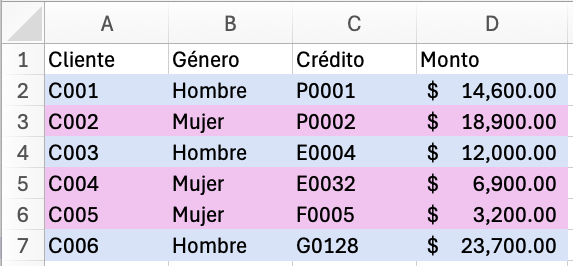
\includegraphics[width=\textwidth]{figures/p101-1.png}
    \end{minipage}
    % \hfill
    % \begin{minipage}{0.4\textwidth}
    %     \centering
    %     \includegraphics[width=\textwidth]{figures/d001.png}
    % \end{minipage}
    % \hfill
    \captionsetup{width=0.9\textwidth}
    \caption{Créditos aprobados a clientes por género}
    \label{fig:p101-1}
\end{figure}
\\
(a) Calcule la suma suma de los montos para hombres y la suma de montos para mujeres usando la fórmula \texttt{=SUMA.SI(RANGO CRITERIO, CRITERIO, RANGO SUMA)}.
\\[6pt]
(b) Calcule la suma suma de los montos para hombres y la suma de montos para mujeres usando la fórmula \texttt{=SUMA(FILTRAR(RANGO SUMA, RANGO INCLUIR))}.

\clearpage

\subsubsection*{Solución al Problema 1}

Para el inciso (a) utilizamos las fórmulas
\\[12pt]
\texttt{=SUMAR.SI(B2:B7,"HOMBRE",D2:D7)}
\\[0pt]
\texttt{=SUMAR.SI(B2:B7,"MUJER",D2:D7)}
\begin{figure}[!ht]
    \centering
    \begin{minipage}{\textwidth}
        \centering
        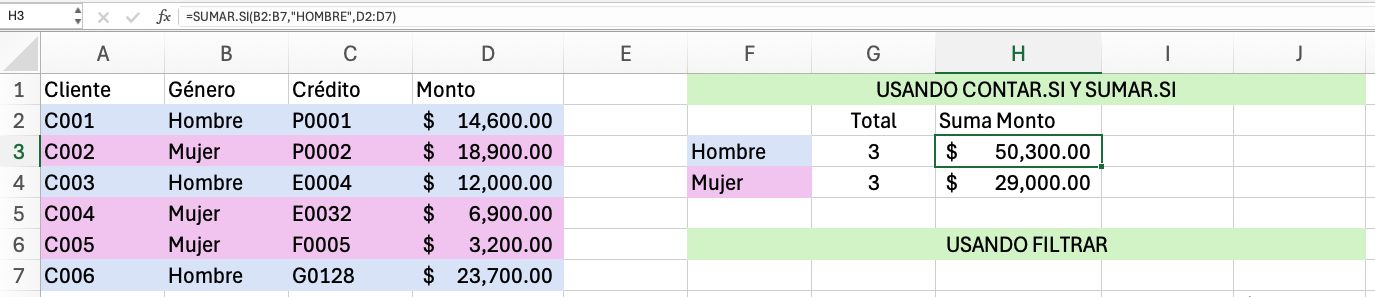
\includegraphics[width=\textwidth]{figures/s101-1a1.png}
    \end{minipage}
    \hfill
    \begin{minipage}{\textwidth}
        \centering
        
\includegraphics[width=\textwidth]{figures/s101-1a2.png}
    \end{minipage}
    \captionsetup{width=0.9\textwidth}
    \caption{Solución al Problema 1 inciso (a)}
    \label{fig:s101-1a}
\end{figure}

\noindent
Para el inciso (b) utilizamos las fórmulas
\\[12pt]
\texttt{=SUMA(FILTRAR(D2:D7,B2:B7="HOMBRE"))}
\\[0pt]
\texttt{=SUMA(FILTRAR(D2:D7,B2:B7="MUJER"))}
\begin{figure}[!ht]
    \centering
    \begin{minipage}{\textwidth}
        \centering
        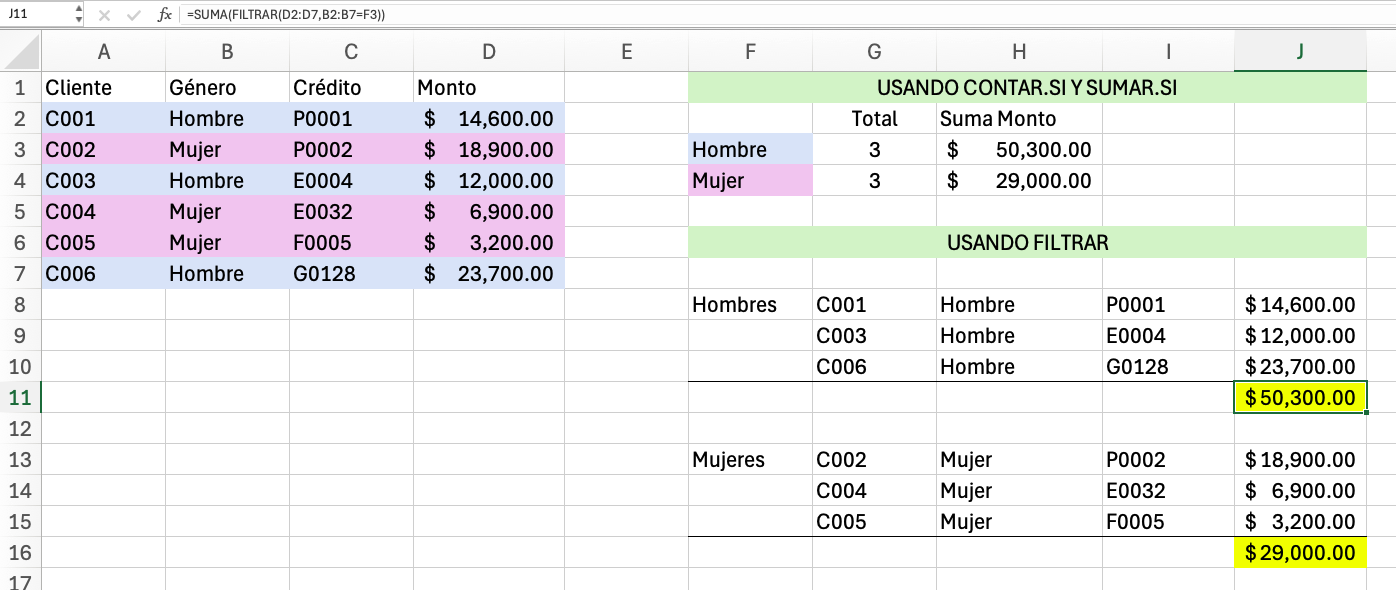
\includegraphics[width=\textwidth]{figures/s101-1b1.png}
    \end{minipage}
    \hfill
    \begin{minipage}{\textwidth}
        \centering
        
\includegraphics[width=\textwidth]{figures/s101-1b2.png}
    \end{minipage}
    \captionsetup{width=0.9\textwidth}
    \caption{Solución al Problema 1 inciso (b)}
    \label{fig:s101-1b}
\end{figure}

\noindent
Nota: Si se utilizamos las fórmulas
\\[12pt]
\texttt{=FILTRAR(A2:D7,B2:B7="HOMBRE")}
\\[0pt]
\texttt{=FILTRAR(A2:D7,B2:B7="HOMBRE")}
\\[12pt]
Se generará la tabla virtual con todos los créditos correspondientes a las filas de los hombres o de las mujeres.
\begin{figure}[!ht]
    \centering
    \begin{minipage}{\textwidth}
        \centering
        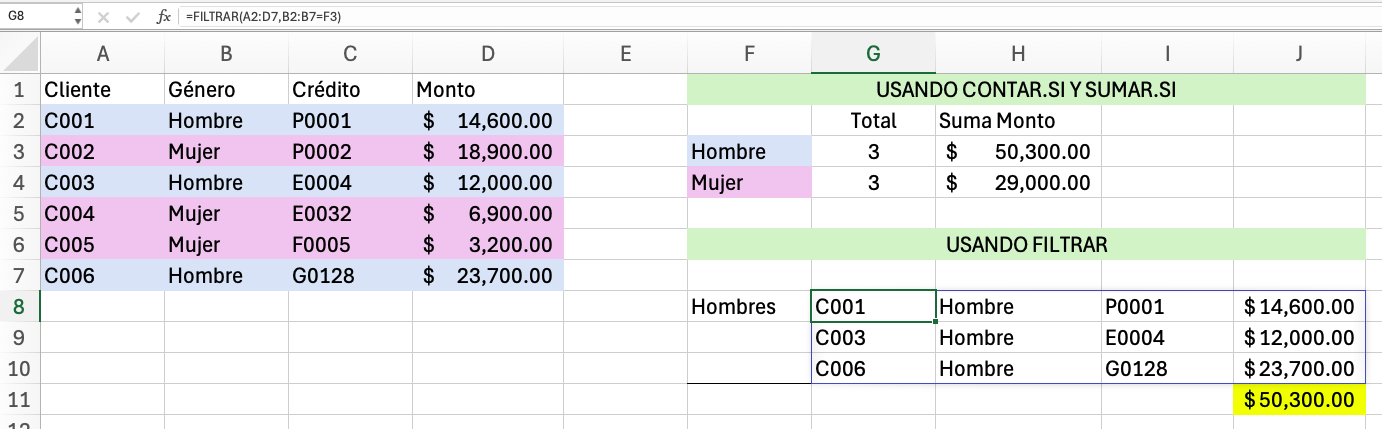
\includegraphics[width=\textwidth]{figures/s101-2.png}
    \end{minipage}
    \hfill
    \begin{minipage}{\textwidth}
        \centering
        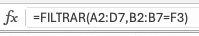
\includegraphics[width=\textwidth]{figures/s101-3.png}
    \end{minipage}
    \hfill
    \begin{minipage}{\textwidth}
        \centering
        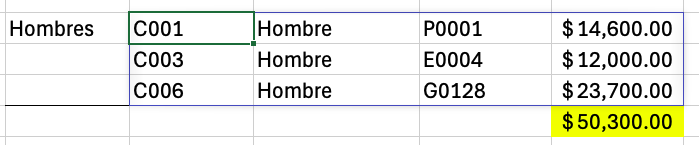
\includegraphics[width=\textwidth]{figures/s101-4.png}
    \end{minipage}
    \captionsetup{width=0.9\textwidth}
    \caption{Tabla virtual generada por FILTRAR (c)}
    \label{fig:s101-c}
\end{figure}

\clearpage

\subsection*{Problema 2 | Uso de Tablas dinámicas en Excel}

Una empresa financiera posee una tabla con los montos de créditos que ha aprobado a sus clientes y su deuda actual. La tabla posee el género de cada cliente y se desea calcular la deuda total y deuda promedio.
\\[12pt]
En la Figura \ref{fig:p102} se muestra la tabla con el cliente, género, crédito, monto aprobado y deuda actual.
\begin{figure}[!ht]
    \centering
    \begin{minipage}{\textwidth}
        \centering
        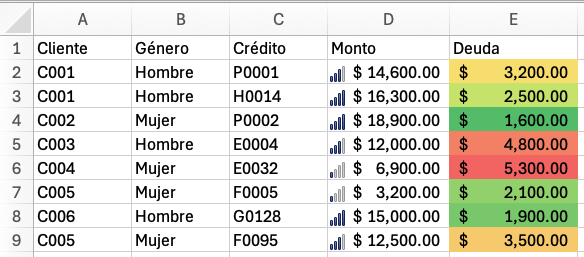
\includegraphics[width=\textwidth]{figures/p102.png}
    \end{minipage}
    % \hfill
    % \begin{minipage}{0.4\textwidth}
    %     \centering
    %     \includegraphics[width=\textwidth]{figures/d001.png}
    % \end{minipage}
    % \hfill
    \captionsetup{width=0.9\textwidth}
    \caption{Créditos aprobados con deuda actual a clientes por género}
    \label{fig:p102}
\end{figure}
\\
(a) Crea una tabla dinámica de \texttt{A1:E9}.
\\[6pt]
(b) Segmenta las filas por Género y luego por Cliente.
\\[6pt]
(c) Cuenta el número de Créditos en valores.
\\[6pt]
(d) Calcula la suma del Monto en valores.
\\[6pt]
(e) Calcula la suma de la Deuda en valores.
\\[6pt]
(f) Calcula el promedio del Monto en valores.
\\[6pt]
(g) Calcula el promedio de la Deuda en valores.
\\[6pt]
(h) ¿Quién es el cliente de mayor deuda?
\\[6pt]
(i) ¿Quién es el cliente al que se le ha prestado más en promedio?
\\[6pt]
(j) ¿Quién es el cliente hombre con mayor deuda promedio?
\\[6pt]
(k) ¿Es significativamente distinta la deuda entre hombres y mujeres?
\\[6pt]
(l) ¿Cuánto se ha recuperado en total de todos los créditos?

\clearpage

\subsubsection*{Solución al Problema 2}

Para el inciso (a) creamos la tabla dinámica para el rango \texttt{A1:E9} y la insertamos en una celda de la misma hoja.
\begin{figure}[!ht]
    \centering
    \begin{minipage}{\textwidth}
        \centering
        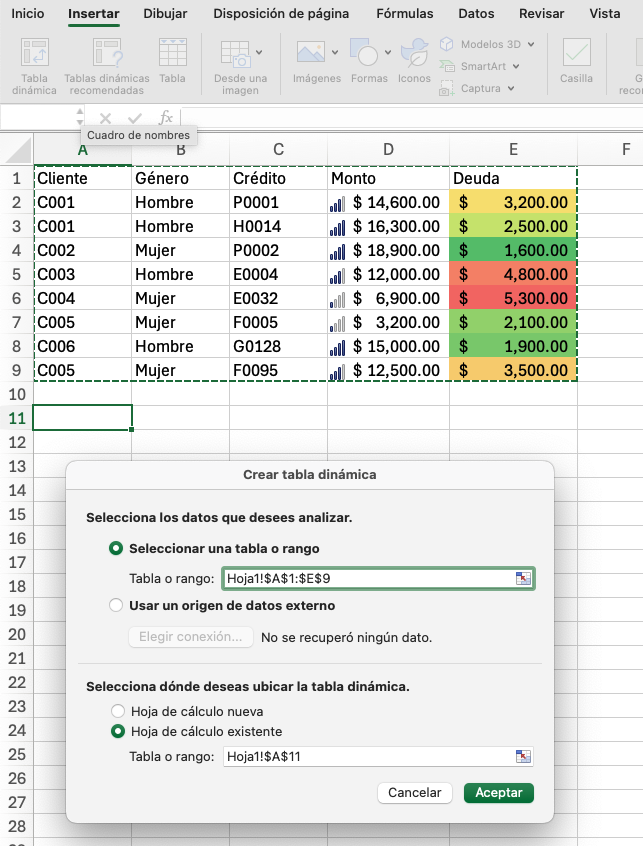
\includegraphics[width=\textwidth]{figures/s102-1.png}
    \end{minipage}
    \captionsetup{width=0.9\textwidth}
    \caption{Solución al Problema 2 inciso (a)}
    \label{fig:s102-1}
\end{figure}

\break
\noindent
Para el inciso (b) arrastramos los campos del género y cliente a las filas
\begin{figure}[!ht]
    \centering
    \begin{minipage}{\textwidth}
        \centering
        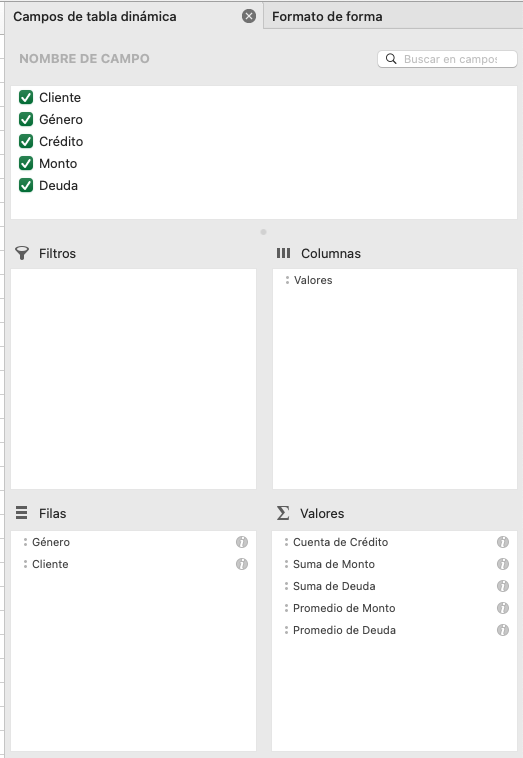
\includegraphics[width=\textwidth]{figures/s102-2.png}
    \end{minipage}
    \captionsetup{width=0.9\textwidth}
    \caption{Solución al Problema 2 inciso (b)}
    \label{fig:s102-2}
\end{figure}

\noindent
Para el inciso (c), (d), (e), (f), (g) arrastramos los campos como valores y configuramos cada campo si es recuento, suma o promedio
\begin{figure}[!ht]
    \centering
    \begin{minipage}{\textwidth}
        \centering
        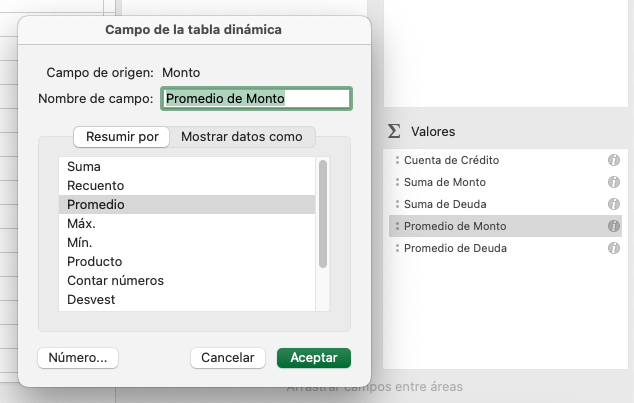
\includegraphics[width=\textwidth]{figures/s102-3.png}
    \end{minipage}
    \captionsetup{width=0.9\textwidth}
    \caption{Solución al Problema 2 incisos (c), (d), (e), (f), (g)}
    \label{fig:s102-3}
\end{figure}

\noindent
Para el inciso (h), (i), (j), (k), (l) observamos los valores en la tabla dinámica
\begin{figure}[!ht]
    \centering
    \begin{minipage}{\textwidth}
        \centering
        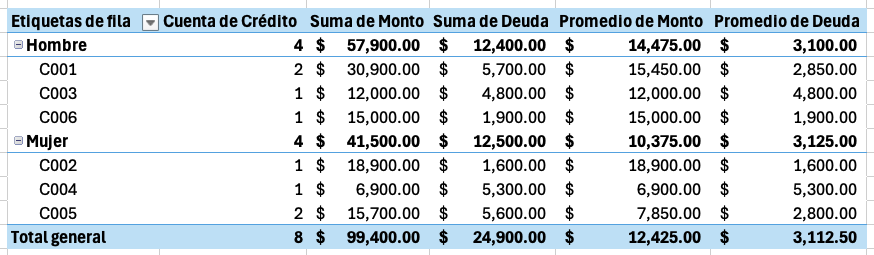
\includegraphics[width=\textwidth]{figures/s102-4.png}
    \end{minipage}
    \captionsetup{width=0.9\textwidth}
    \caption{Solución al Problema 2 incisos (h), (i), (j), (k), (l)}
    \label{fig:s102-4}
\end{figure}

\noindent
Respuestas: (h) \textbf{C001 \$5,700}, (i) \textbf{C002 \$18,900}, (j) \textbf{C003 \$4,800}, (k) \textbf{No, la diferencia es de \$100 menor al 1\% de diferencia}, (l) \textbf{\$74,500 = \$99,400 - \$24,900}.

\clearpage

\subsection*{Problema 3 | Uso de Power BI}

Una empresa financiera posee una tabla con los préstamos que ha aprobado a sus clientes indicando el monto, el estado y el valor. En cada préstamo se reporta el estado de sobre lo que se ha pagado del préstamo, lo que se debió haber cubierto actualmente (deuda) y lo que se debería cubrir en el futuro (pendiente). La financiera requiere una tabla que resuma de cada cliente sus préstamos y en cada préstamo se desglose la suma de cuánto adeuda, cuánto ha pagado y cuánto está pendiente, así como el total. También requiere un indicador que muestre la diferencia entre la suma del monto del préstamo y el valor del monto pagado, para saber cuánto se adeuda en total del préstamo, igualmente desglosado por cliente y préstamo. Finalmente la financiera requiere dos reportes visuales, un anillo que muestre el estado de los préstamos (pagado, pendiente y deuda) segmentado por cliente. Y un esquema jerárquico que permita desglosar el valor del préstamo por su estado, cliente y número de préstamo.
\\[12pt]
En la Figura \ref{fig:p103} se muestra la tabla de préstamos, con la columna del cliente, el número de préstamo, el monto, el estado (pagado, deuda, pendiente) y el valor asociado al estado.
\begin{figure}[!ht]
    \centering
    \begin{minipage}{\textwidth}
        \centering
        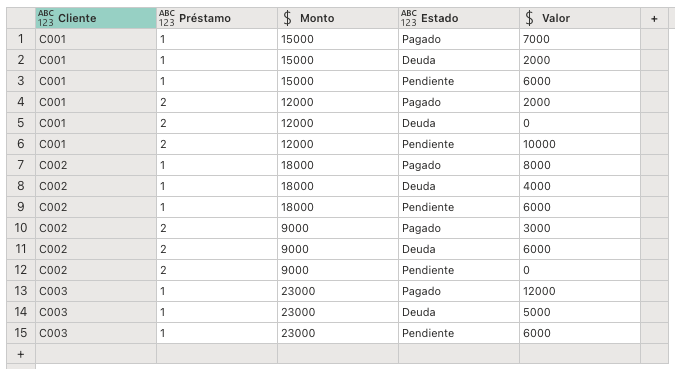
\includegraphics[width=\textwidth]{figures/p103.png}
    \end{minipage}
    \captionsetup{width=0.9\textwidth}
    \caption{Préstamos aprobados a clientes desglosado por cliente, número de préstamo, estado (pagado, deuda y pendiente) y valor asociado al estado}
    \label{fig:p103}
\end{figure}
\\

\break
\noindent
(a) Crea una matriz que reporte las filas para el cliente y número de préstamo en ese orden, el estado como columna y la suma del valor en los valores.
\\[6pt]
(b) En el modelo de datos crea una nueva medida con la fórmula
\\[6pt]
\texttt{Diferencia = SUM(P103[Monto])-SUM(P103[Valor])} 
\\[6pt]
para reportar la diferencia entre la suma del monto menos la suma del valor asociado al estado. Donde \textit{P103} es el nombre de la tabla creada al inicio.
\\[6pt]
(c) Crea una matriz que reporte las filas para el cliente y número de préstamo en ese orden, el estado como columna y la suma del monto, suma del valor y suma de diferencia en los valores en ese orden. Reporta solo el estado Pagado en los filtros del objeto visual.
\\[6pt]
(d) Crea una gráfica de anillo cuya leyenda este dada por el estado del préstamo, en valores reporte la suma del valor asociado al estado, y en detalles segmente al cliente.
\\[6pt]
(e) Crea un esquema jerárquico para analizar la suma del valor valor asociado al estado, explicado por el estado del préstamo, el cliente y el número de préstamo en ese orden.
\\[6pt]
(f) De la matriz del inciso (a) responde si cada desglose corresponde al monto reportado en cada préstamo.
\\[6pt]
(g) De la matriz del inciso (b) responde cuál el es el préstamo con menor deuda total y usando el inciso (a) cómo es su deuda respecto al préstamo.
\\[6pt]
(h) Del anillo identifica al cliente de mayor deuda y el cliente con mayor valor pendiente.
\\[6pt]
(i) Del esquema jerárquico identifica al cliente de mayor deuda y el número de préstamo de mayor deuda para ese cliente.

\clearpage

\subsubsection*{Solución al Problema 3}

Para el inciso (a) creamos una matriz que reporte las filas para el cliente y número de préstamo en ese orden, el estado como columna y la suma del valor en los valores.
\begin{figure}[!ht]
    \centering
    \begin{minipage}{\textwidth}
        \centering
        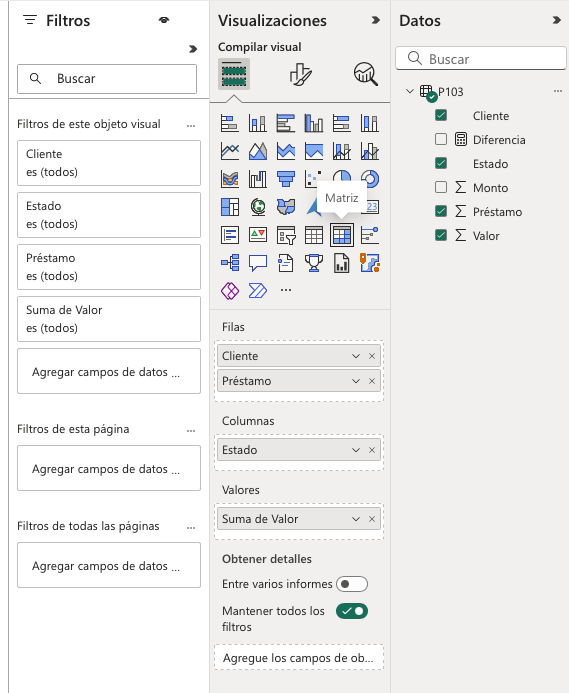
\includegraphics[width=0.7\textwidth]{figures/s103a-1.png}
    \end{minipage}
    \hfill
    \begin{minipage}{\textwidth}
        \centering
        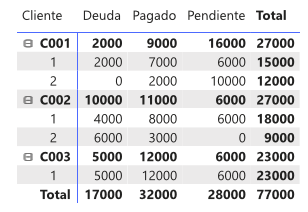
\includegraphics[width=0.7\textwidth]{figures/s103a-2.png}
    \end{minipage}
    \captionsetup{width=0.9\textwidth}
    \caption{Solución al Problema 3 inciso (a)}
    \label{fig:s103a}
\end{figure}

\noindent
Para el inciso (b) abrimos el modelo de datos y dentro del modelo de datos creamos una nueva medida con la fórmula para calcular la diferencia.
\begin{figure}[!ht]
    \centering
    \begin{minipage}{\textwidth}
        \centering
        
\includegraphics[width=\textwidth]{figures/s103b-1.png}
    \end{minipage}
    \hfill
    \begin{minipage}{\textwidth}
        \centering
        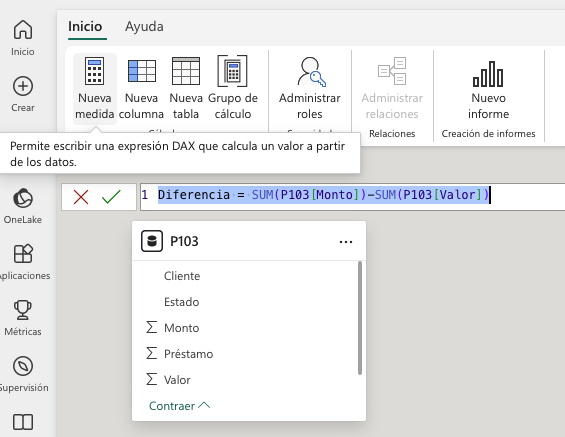
\includegraphics[width=\textwidth]{figures/s103b-2.png}
    \end{minipage}
    \hfill
    \begin{minipage}{\textwidth}
        \centering
        
\includegraphics[width=\textwidth]{figures/s103b-3.png}
    \end{minipage}
    \captionsetup{width=0.9\textwidth}
    \caption{Solución al Problema 3 inciso (b)}
    \label{fig:s103b}
\end{figure}

\break
\noindent
Para el inciso (c) creamos una matriz que reporte las filas para el cliente y número de préstamo en ese orden, el estado como columna y la suma del monto, suma del valor y suma de diferencia en los valores en ese orden. Reporta solo el estado Pagado en los filtros del objeto visual.
\begin{figure}[!ht]
    \centering
    \begin{minipage}{\textwidth}
        \centering
        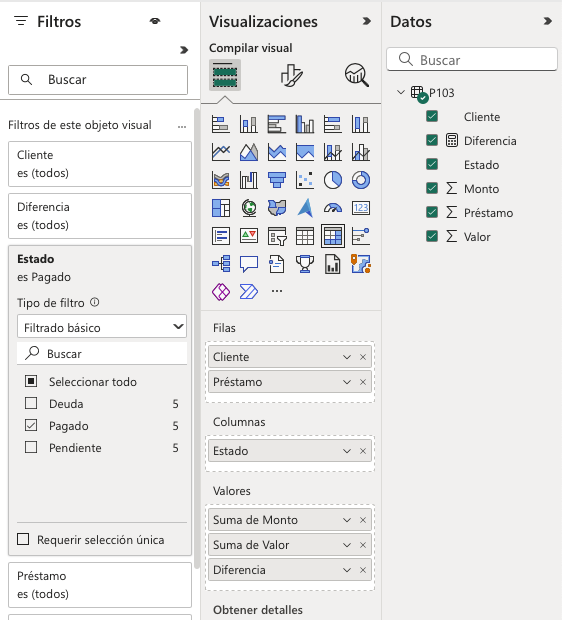
\includegraphics[width=0.9\textwidth]{figures/s103c-1.png}
    \end{minipage}
    \hfill
    \begin{minipage}{\textwidth}
        \centering
        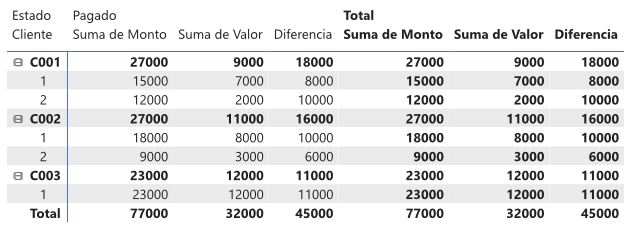
\includegraphics[width=0.9\textwidth]{figures/s103c-2.png}
    \end{minipage}
    \captionsetup{width=0.9\textwidth}
    \caption{Solución al Problema 3 inciso (c)}
    \label{fig:s103c}
\end{figure}

\noindent
Para el inciso (d) creamos una gráfica de anillo cuya leyenda este dada por el estado del préstamo, en valores reporte la suma del valor asociado al estado, y en detalles segmente al cliente.
\begin{figure}[!ht]
    \centering
    \begin{minipage}{\textwidth}
        \centering
        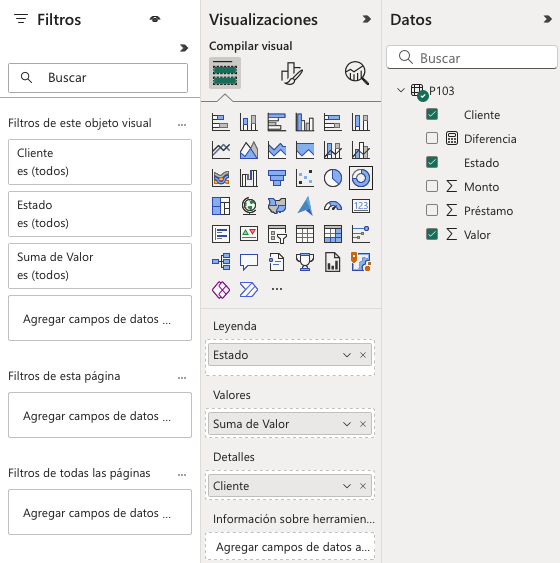
\includegraphics[width=0.8\textwidth]{figures/s103d-1.png}
    \end{minipage}
    \hfill
    \begin{minipage}{\textwidth}
        \centering
        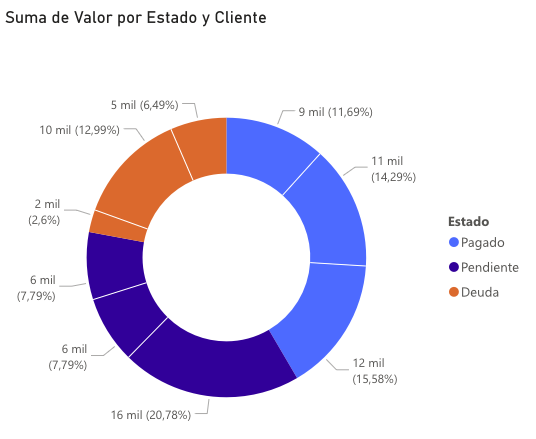
\includegraphics[width=0.7\textwidth]{figures/s103d-2.png}
    \end{minipage}
    \captionsetup{width=0.9\textwidth}
    \caption{Solución al Problema 3 inciso (d)}
    \label{fig:s103d}
\end{figure}

\noindent
Para el inciso (e) creamos un esquema jerárquico para analizar la suma del valor valor asociado al estado, explicado por el estado del préstamo, el cliente y el número de préstamo en ese orden.
\begin{figure}[!ht]
    \centering
    \begin{minipage}{\textwidth}
        \centering
        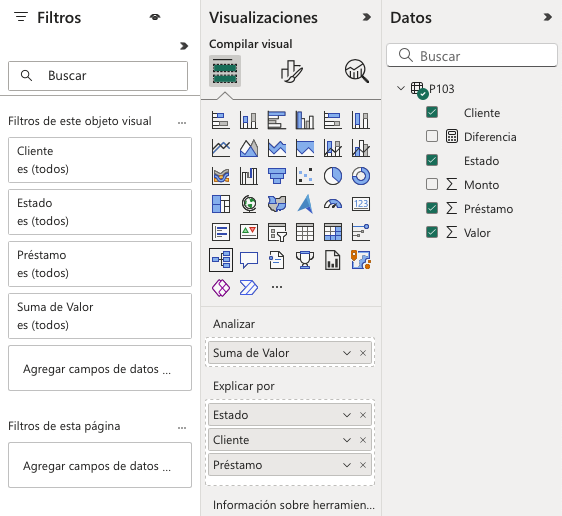
\includegraphics[width=0.9\textwidth]{figures/s103e-1.png}
    \end{minipage}
    \hfill
    \begin{minipage}{\textwidth}
        \centering
        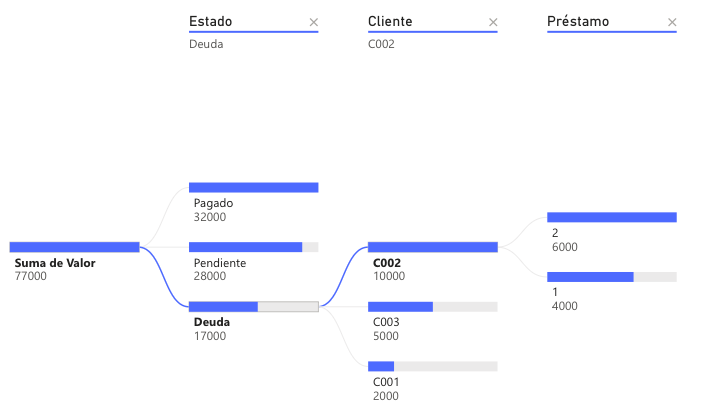
\includegraphics[width=0.9\textwidth]{figures/s103e-2.png}
    \end{minipage}
    \captionsetup{width=0.9\textwidth}
    \caption{Solución al Problema 3 inciso (e)}
    \label{fig:s103e}
\end{figure}

\noindent
Para los otros incisos las respuestas son: (f) Sí, la suma de montos en cada préstamo coincide con la suma de su deuda, lo pagado y lo pendiente. (g) Para el cliente \textit{C002} en el préstamo número \textit{2} la diferencia total es de \textbf{\$6,000} y es el préstamo de menor deuda, ya que lo pendiente para ese préstamo es de \textbf{\$0}, sin embargo, respecto a los otros préstamos es el de mayor deuda. (h) \textbf{C002 \$10,000 12.99\%} es el cliente de mayor deuda y \textbf{C001 \$16,000 20.78\%} es el cliente de mayor valor pendiente. (i) \textbf{C002 \$10,000 2 \$10,000} es el cliente de mayor deuda, con su préstamo número dos.

\clearpage

\subsection*{Problema 4 | Uso de Python}

Un banco ha decidido usar Python en un ambiente controlado para poder hacer operaciones y cálculos de riesgo, para ello ha instalado un ambiente virtual cerrado en computadoras sin acceso a internet para que no se filtren los conjuntos de datos utilizados, ni los reportes generados.
\\[12pt]
El banco comenzará por automatizar una serie de funciones útiles que pueda aplicar para cálculos simples, para de esta forma crear una metodología de trabajo cuando deseen incrementar el volumen de las operaciones.
\\[12pt]
Para ello, el banco requiere que se generen los siguientes reportes automatizados para saber que todo está funcionando correctamente.
\\[12pt]
Implementa las funciones que se detallan a continuación y resuelve los incisos siguietes. Completa el código que haga falta para que las funciones operen correctamente siguiendo las pistas de los comentarios
\scriptsize
\begin{verbatim}
def reporteTitulo(codigo, leyenda):
    print(f"Banco Nacional - Reporte {codigo} / {leyenda}")

def reporteCorte(codigo, leyenda):
    print(f"-------------- {codigo} / {leyenda} --------------")

def reporteFin(codigo, leyenda):
    print(f"-------------- {codigo} / {leyenda} --------------")

def reporteBalanceDiaInicio(balance):
    reporteTitulo("BIN", "Balance al Inicio del Día")
    print(f"$ {balance:.2f}")
    reporteFin("BIN", "Balance al Inicio del Día")

def reporteBalanceDiaFin(balance):
    reporteTitulo("B-OUT", "Balance al Final del Día")
    print(f"$ {balance:.2f}")
    reporteFin("B-OUT", "Balance al Final del Día")

def reporteTotalOperacionesDia(numOperaciones):
    reporteTitulo("T-OP", "Total de Operaciones del Día")
    # Imprime el número de operaciones
    reporteFin("T-OP", "Total de Operaciones del Día")

def reporteTotalOperacionesRelativasMes(numOperacionesDia, numOperacionesMes):
    reporteTitulo("T-OR", "Tasa de Operaciones del día respecto al mes")
    tasa = 100 * numOperacionesDia / numOperacionesMes
    # Imprime el número de operaciones del dia
    # luego una diagonal y el número de operaciones del mes
    # Haz un corte del reporte
    # Imprime la tasa de operaciones del día respecto al mes a un dígito
    # Ejemplo: 41/200 (20.5%)
    reporteFin("T-OR", "Tasa de Operaciones del día respecto al mes")
\end{verbatim}
\hfill
\normalsize

\noindent
(a) Reporta el balance de inicio del día con \textbf{\$ 185,000.32}
\\[6pt]
(b) Reporta un total de \textbf{247} operaciones del día
\\[6pt]
(c) Reporta un total de \textbf{247} de \textbf{192,316} operaciones relativas del mes
\\[6pt]
(d) Reporta el balance de fin del día con \textbf{\$ 232,827.71}
\\[6pt]

\clearpage

\subsubsection*{Solución al Problema 4}

En este problema se presetan una serie de funciones que hacen impresiones en la pantalla con los parámetros que se les mande. Las funciones son sencillas y solo reciben parámetros de texto o números para imprimir en la pantalla algunos cortes.
\\[12pt]
En la Figura \ref{fig:s104-1} se muestra el código completado donde hemos colocado los \texttt{print} faltantes para que se muestren los reportes correctamente.
\begin{figure}[!ht]
    \centering
    \begin{minipage}{\textwidth}
        \centering
        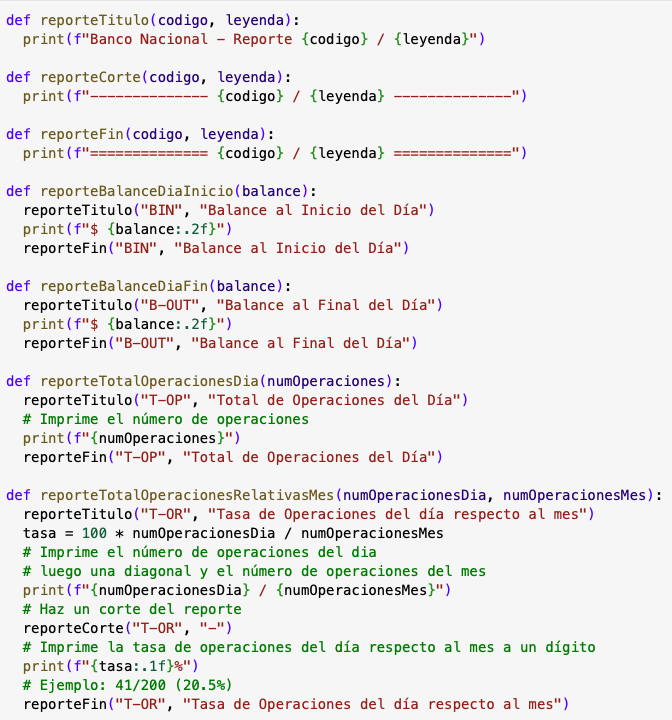
\includegraphics[width=\textwidth]{figures/s104-1.png}
    \end{minipage}
    \captionsetup{width=0.9\textwidth}
    \caption{Código solucionado, se agregan impresiones faltantes}
    \label{fig:s104-1}
\end{figure}

\break
\noindent
En la Figura \ref{fig:s104-2} se muestra el código para resolver los incisos (a), (b), (c) y (d) que únicamente solicitan llamar a las funciones con los valores establecidos en cada inciso.
\begin{figure}[!ht]
    \centering
    \begin{minipage}{\textwidth}
        \centering
        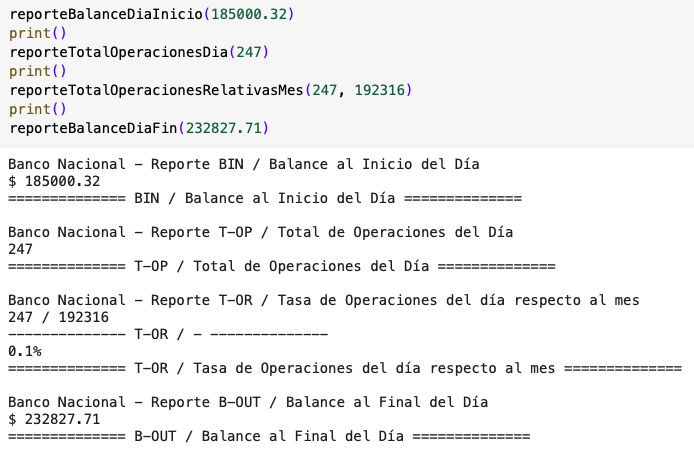
\includegraphics[width=\textwidth]{figures/s104-2.png}
    \end{minipage}
    \captionsetup{width=0.9\textwidth}
    \caption{Código para resolver los incisos}
    \label{fig:s104-2}
\end{figure}

\clearpage

\subsection*{Problema 5 | Interés Simple}

Una financiera posee montos de préstamos a proyectos y la tasa anual fija que le cobrará sus clientes. La financiera requiere calcular la suma de montos y proponer una misma tasa de interés anual única para todos los proyectos, así como encontrar la tasa anual en caso de perder el monto por algún proyecto.
\\[12pt]
En la Figura \ref{fig:p105} se muestran los montos y la tasa anual de los montos de préstamo destinados a proyectos financiados.
\begin{figure}[!ht]
    \centering
    \begin{minipage}{\textwidth}
        \centering
        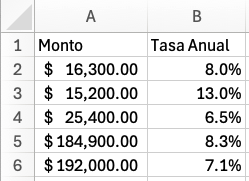
\includegraphics[width=\textwidth]{figures/p105.png}
    \end{minipage}
    \captionsetup{width=0.9\textwidth}
    \caption{Montos de préstamos a proyectos de una financiera y su tasa anual}
    \label{fig:p105}
\end{figure}
\\

\noindent
(a) Calcula el interés simple generado por la tasa anual y reporta cada interés y la suma de todos estos intereses. 
\\[6pt]
(b) Calcula la tasa anual promedio y de todas las tasas y la suma de todos los montos y calcula el interés de la suma total con la tasa anual promedio. ¿Este interés es el mismo que el del la suma del inciso (a)?
\\[6pt]
(c) ¿Cuál debería ser la tasa anual de todos los montos para que la suma del interés sea la misma?
\\[6pt]
(d) ¿Cuál debería ser la tasa anual de todos los montos, si no existiera el monto de \textbf{\$ 25,400.00} para que la suma del interés sea la misma a las anteriores?

\clearpage

\subsubsection*{Solución al Problema 5}

En este problema nos muestran una tabla de montos y tasas anuales y debemos cacular el interés de cada monto según su tasa y la suma de estos intereses.
\\[12pt]
En la Figura \ref{fig:s105-1} se muestra el código que define los montos y tasas como listas, luego inicializa un total que sumará los intereses comenzando en cero, y luego se recorre cada pareja de monto y tasa usando la función de agrupado o embolsado llamada \texttt{zip}. Luego, dentro del iterador, calculamos los intereses del monto, según su tasa y los acumulamos en el total, finalmente se hacen las impresiones necesarias para reportar el monto, su tasa, el interés y al final la suma de todos los intereses.
\begin{figure}[!ht]
    \centering
    \begin{minipage}{\textwidth}
        \centering
        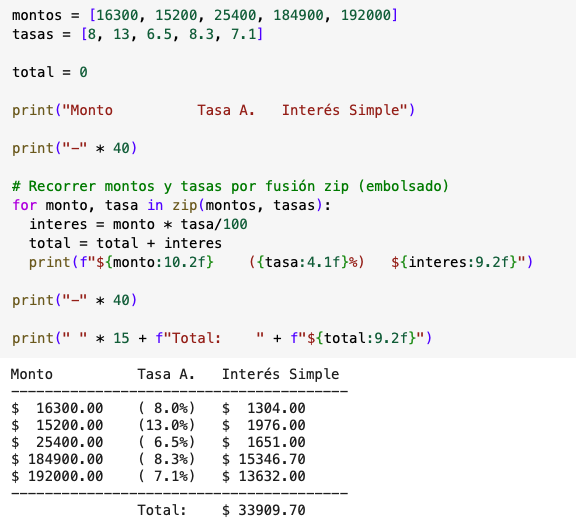
\includegraphics[width=\textwidth]{figures/s105-1.png}
    \end{minipage}
    \captionsetup{width=0.9\textwidth}
    \caption{Código para reportar el interés de montos y tasas con su total final, resultado de la suma de intereses}
    \label{fig:s105-1}
\end{figure}

\break
\noindent
En la Figura \ref{fig:s105-2} se muestra el código que resuelve los incisos (b), (c) y (d). Observa que al promediar la suma de intereses no es igual y que podemos calcular la tasa promedio analíticamente.
\begin{figure}[!ht]
    \centering
    \begin{minipage}{\textwidth}
        \centering
        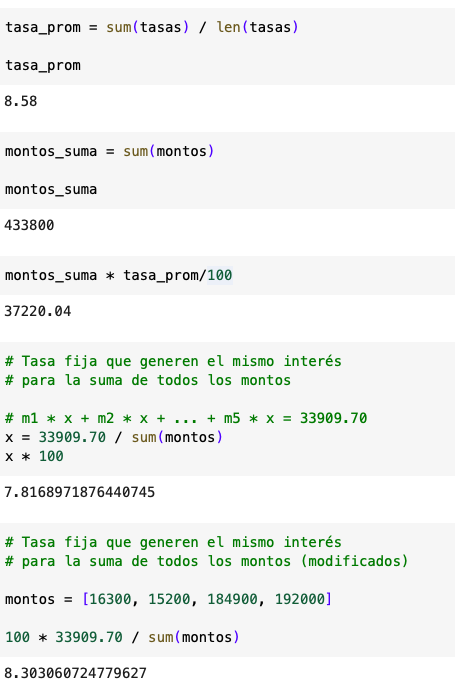
\includegraphics[width=0.9\textwidth]{figures/s105-2.png}
    \end{minipage}
    \captionsetup{width=0.9\textwidth}
    \caption{Código para resolver los incisos}
    \label{fig:s105-2}
\end{figure}

\clearpage

\subsection*{Problema 6 | Interés Compuesto}

Una financiera desea calcular el interés compuesto que generaría un monto de \textbf{\$ 4,312,939.83} con una tasa anual de \textbf{8\%}, si se tuviera que pagar mensualmente a una tasa compuesta de \textbf{0.67\%} y si tuviera que pagar a tasa compuesta de \textbf{0.34\%}.
\\[12pt]
(a) Calcula el interés compuesto a 12 meses con una tasa mensual de \textbf{0.67\%}. 
\\[6pt]
(b) Calcula el interés compuesto a 24 quincenas con una tasa quincenal de \textbf{0.34\%}

\clearpage

\subsubsection*{Solución al Problema 6}

En este problema nos pide calcular el interés compuesto al 12 meses y 24 quincenas para compararlo con el interés simple. El interés calcula los intereses periodo por periodo y los va acumulando en un nuevo monto sobre el que se calculará el nuevo interés. Este procedimiento es importante para algunas financieras que contemplan incrementos al monto por pagos tardíos o penalizaciones haciendo que se recupere el riesgo ocurrido en cada periodo sin tener que fijar un único interés sobre todo el el monto inicial.
\\[12pt]
En la Figura \ref{fig:s106-1} se muestra el código para calcular el interés simple del monto respecto a la tasa anual, y luego el codigo para ir calculando mes por mes el interés compuesto. El código se puede adaptar fácilmente para calcular los intereses quincenales en lugar de los mensuales, considerando ahora 24 periodos. Observa como se define una variable que guarde el monto acumulado y como se calcula el interés mes por mes para ese monto acumulado. También se usa \texttt{mes + 1} porque \texttt{range(12)} genera 12 iteraciones desde 0 hasta 11.
\begin{figure}[!ht]
    \centering
    \begin{minipage}{\textwidth}
        \centering
        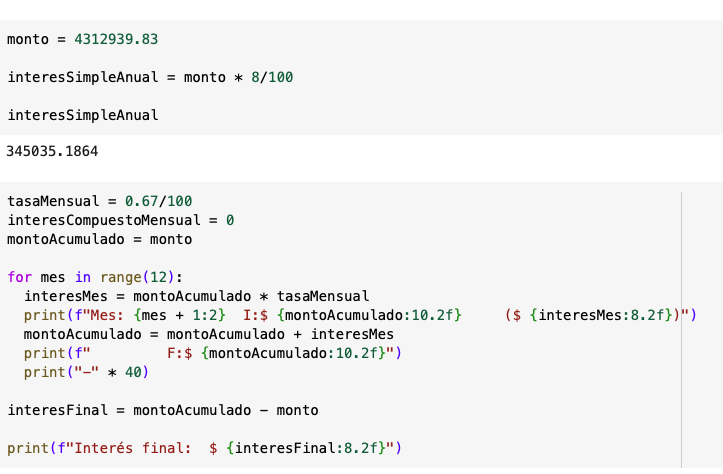
\includegraphics[width=\textwidth]{figures/s106-1.png}
    \end{minipage}
    \captionsetup{width=0.9\textwidth}
    \caption{Código para generar los intereses mensuales compuestos}
    \label{fig:s106-1}
\end{figure}

\break
\noindent
En la Figura \ref{fig:s106-2} se muestra el reporte generado por el código, mostrando cual es el monto acumulado al inicio y al final y el interes que se calcula. Además se muestra al final el último interés calculado que es el interés compuesto final.
\begin{figure}[!ht]
    \centering
    \begin{minipage}{\textwidth}
        \centering
        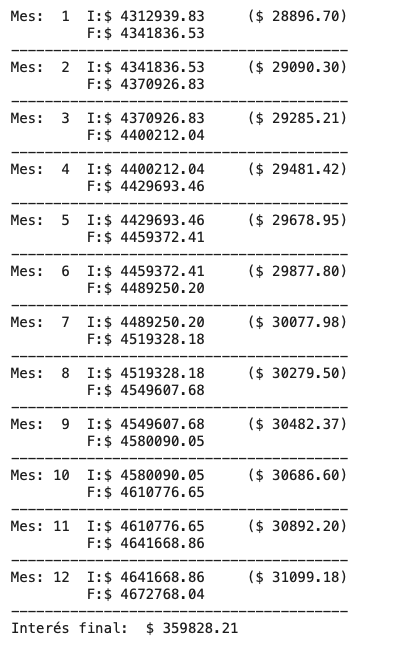
\includegraphics[width=0.8\textwidth]{figures/s106-2.png}
    \end{minipage}
    \captionsetup{width=0.9\textwidth}
    \caption{Reporte de intereses acumulados en 12 meses}
    \label{fig:s106-2}
\end{figure}

\break
\noindent
En la Figura \ref{fig:s106-3} se muestra el código para generar de forma analítica el interés compuesto a 12 meses. Luego se muestra la solución al inciso (b) ya sin generar la tabla, solo reportar el interés compuesto para las 24 quincenas.
\begin{figure}[!ht]
    \centering
    \begin{minipage}{\textwidth}
        \centering
        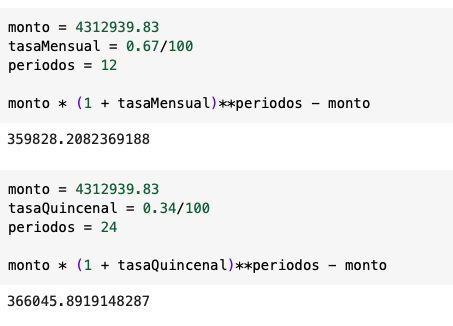
\includegraphics[width=0.8\textwidth]{figures/s106-3.png}
    \end{minipage}
    \captionsetup{width=0.9\textwidth}
    \caption{Intereses acumuladoss en 12 meses y en 24 quincenas}
    \label{fig:s106-3}
\end{figure}

\clearpage

\subsection*{Problema 7 | Tasa de Interés Variable}

Una financiera desea calcular el interés que generaría un monto de \textbf{\$ 2,617,800.01} con una tasa mensual variable que comienza en \textbf{6\%} el primer mes y se actualiza a \textbf{5\%} para el segundo mes, luego \textbf{4\%} al tercer mes, \textbf{3\%} para el cuarto mes y luego \textbf{2\%} y \textbf{1\%} para el quinto y sexto mes, luego de ahí se aplica el \textbf{0.5\%} en los meses restantes.
\\[12pt]
(a) Calcula el interés compuesto para los 12 meses usando el interés variable. 
\\[6pt]
(b) Si se usara un interés anual fijo, ¿De cuánto sería?

\clearpage

\subsubsection*{Solución al Problema 7}

En este problema nos pide calcular el interés variable donde mes con més el interés varía según alguna regla establecida, por ejemplo, para que los primeros meses el interés sea alto y luego se regule. Esto ayuda a financieras y prestamistas para que recuperen rápidamente el capital invertido en los primeros meses y luego se arrieguen a que el cliente que ya no pague no genere una pérdida fuerte para la empresa tras quedarse el bien adquirido a meses.
\\[12pt]
En la Figura \ref{fig:s107-1} se muestra el código para calcular el interés variable que se va acumulando, muy similar al problema del interés acumulado, pero ahora considerando la regla de variación del interés dada por el contador y la condición especial para que a partir del mes 7 equivalente a que el contador llegue a cero, de que el interés se regule.
\begin{figure}[!ht]
    \centering
    \begin{minipage}{\textwidth}
        \centering
        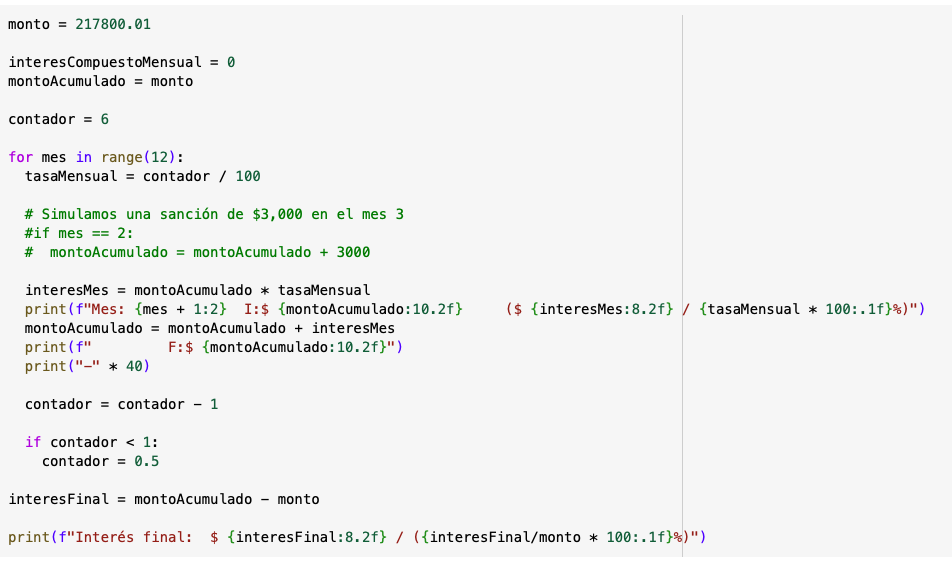
\includegraphics[width=\textwidth]{figures/s107-1.png}
    \end{minipage}
    \captionsetup{width=\textwidth}
    \caption{Código para generar los intereses variables compuestos mensuales}
    \label{fig:s107-1}
\end{figure}

\break
\noindent
En la Figura \ref{fig:s107-2} se muestra el reporte generado por el código, mostrando el monto acumulado y el interés que va variando mes con mes hasta regularizarse en los últimos meses como lo pide el problema.
\begin{figure}[!ht]
    \centering
    \begin{minipage}{\textwidth}
        \centering
        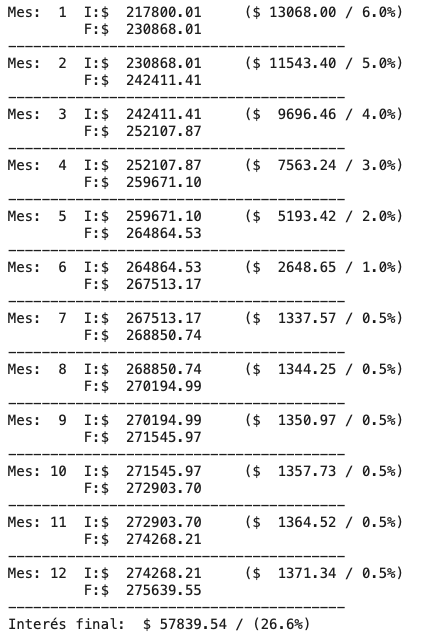
\includegraphics[width=0.9\textwidth]{figures/s107-2.png}
    \end{minipage}
    \captionsetup{width=0.9\textwidth}
    \caption{Reporte de intereses variables acumulados en 12 meses}
    \label{fig:s107-2}
\end{figure}

\clearpage

\subsection*{Problema 8 | Tabla de Amortización Simple}

Una financiera desea calcular una tabla de amortización para un monto financiado de \textbf{\$ 6,500.00}, con un enganche inicial de \textbf{\$ 2,300.00}, el cual pagará los intereses amortizados. Los intereses están diseñados para que bajen linealmente durante 48 semanas y recuperen \textbf{80\%} del monto financiado. Es decir, se necesitan recuperar intereses por el \textbf{80\%} de los \textbf{\$ 6,500.00}, diseñando intereses que se reduzcan linealmente en 48 pagos y luego se considere el enganche inicial como descuento inmediato a los primeros intereses.
\\[12pt]
(a) Calcula la tabla de amortización sin considerar el enganche.
\\[6pt]
(b) ¿Cuántos pagos iniciales cubre el enganche?
\\[6pt]
(c) Determina un abono fijo para terminar de pagar los intereses más el monto financiado en 48 semanas.

\clearpage

\subsubsection*{Solución al Problema 8}

En este problema nos pide construir una tabla de amortización indicando el abono fijo y la parte de intereses.
\\[12pt]
En la Figura \ref{fig:s108-1} se muestra el código para describir el problema, especificar el monto y calcular los intereses esperados por el cliente y el total que terminará pagando, así como reporte generado.
\begin{figure}[!ht]
    \centering
    \begin{minipage}{\textwidth}
        \centering
        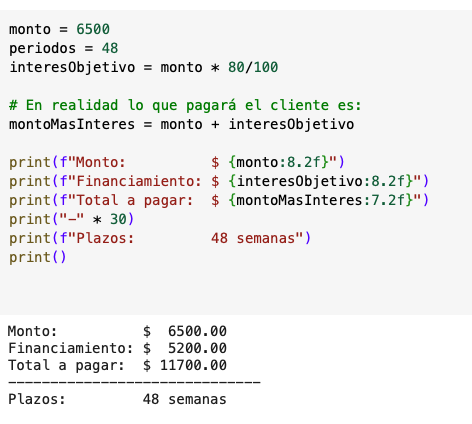
\includegraphics[width=\textwidth]{figures/s108-1.png}
    \end{minipage}
    \captionsetup{width=\textwidth}
    \caption{Código para describir el problema de la amortización}
    \label{fig:s108-1}
\end{figure}

\break
\noindent
En la Figura \ref{fig:s108-2} se muestra el código que calcula el abono fijo sobre el monto que se distribuirá en los 48 meses, luego el monto acumulado, seguido de un valor de amortización, este valor puede ser cualquiera, y se debe ir ajustando hasta que el monto acumulado sea el mismo al total esperado que se desea alcanzar al mes 48, en este caso se partió de un valor inicial de \textbf{\$1,000}, el cual se pasaba y se fue ajustando hasta encontrar el valor de \textbf{\$285.233} que daba una solución exacta a dos dígitos para alcanzar los \textbf{\$11,700.00} esperados. Se describe también el factor de amortización, que será el que determine cuánto se reducirán los intereses mes con mes, en este caso el mes siguiente tendrá intereses por el \textbf{95\%} del mes anterior. Dentro del iterador se calcula el pago que deberá realizar el cliente en cada mes, el monto que se va acumulando y el interés amortizado actualizado.
\begin{figure}[!ht]
    \centering
    \begin{minipage}{\textwidth}
        \centering
        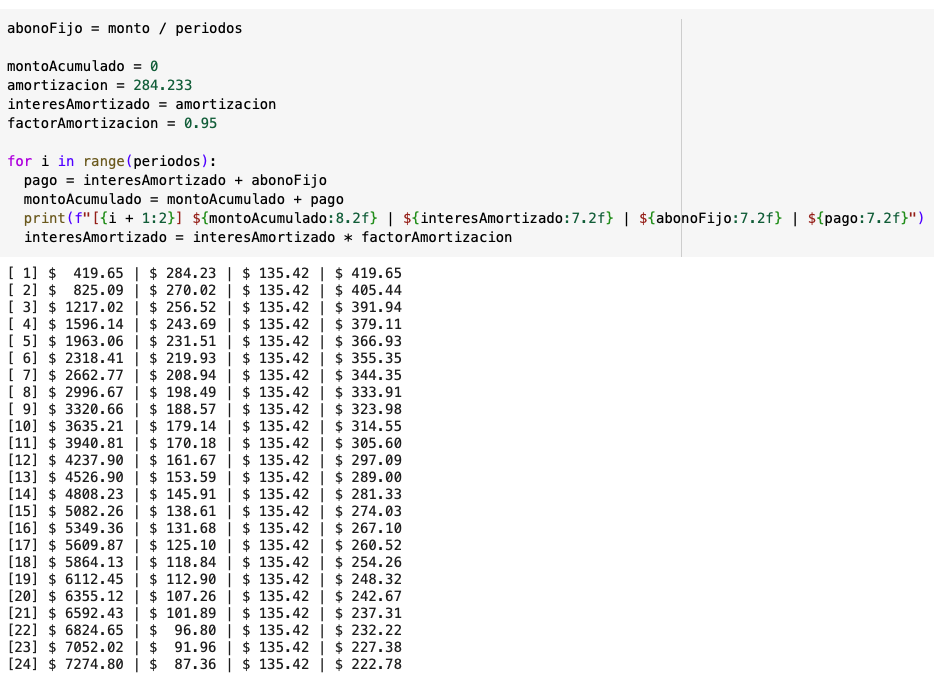
\includegraphics[width=\textwidth]{figures/s108-2.png}
    \end{minipage}
    \captionsetup{width=0.9\textwidth}
    \caption{Código para generar la tabla de amortización con sus primeros resultados}
    \label{fig:s108-2}
\end{figure}

\break
\noindent
En la Figura \ref{fig:s108-3} se muestra la otra parte del reporte para los últimos meses, observando que efectivamente al mes 48 el cliente ha pagado un acumulado de \textbf{\$11,700.00}.
\begin{figure}[!ht]
    \centering
    \begin{minipage}{\textwidth}
        \centering
        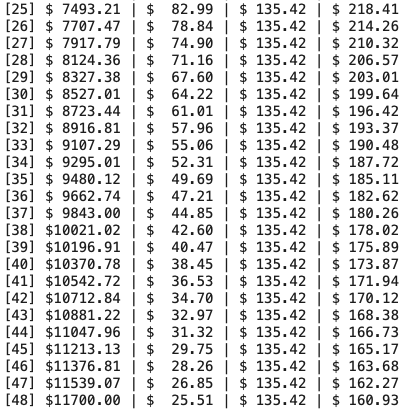
\includegraphics[width=\textwidth]{figures/s108-3.png}
    \end{minipage}
    \captionsetup{width=0.9\textwidth}
    \caption{Reporte de amortización para los últimos meses}
    \label{fig:s108-3}
\end{figure}

\clearpage

\subsection*{Problema 9 | Interés Simple Futuro}

Un banco financió un proyecto durante 36 meses por \textbf{\$ 8,496,500.00}, con una tasa anual fija y simple del \textbf{12\%} y desea calcular los intereses que se generarán al mes 25 y al mes 30. También desea saber en qué mes los intereses superarán el valor de los \textbf{\$ 40,000.00}.
\\[12pt]
(a) Calcula los intereses para el mes 25 y 30.
\\[6pt]
(b) Determina en qué mes los intereses superarán los \textbf{\$ 40,000.00}.
\\[6pt]
(c) Calcula el valor de las cuotas fijas para cubrir el préstamos en los 36 meses.
\\[6pt]
(d) Calcula el valor de las cuotas fijas para cubrir el préstamos en los 36 meses, si se da un adelanto del \textbf{10\%} del valor del proyecto (los intereses deberían ser los mismos).

\clearpage

\subsubsection*{Solución al Problema 9}

En este problema nos pide calcular el interés futuruo para el mes 25 y 30 usando el interés simple. Esto lo podemos hacer proyectando los meses futuros entre 12 meses que tiene el año ya que la tasa es anual. 
\\[12pt]
En la Figura \ref{fig:s109-1} se muestra el código que calcula los intereses anuales y los futuros para el total de meses. Observa que con una proyección de los periodos entre 12 se consigue.
\begin{figure}[!ht]
    \centering
    \begin{minipage}{\textwidth}
        \centering
        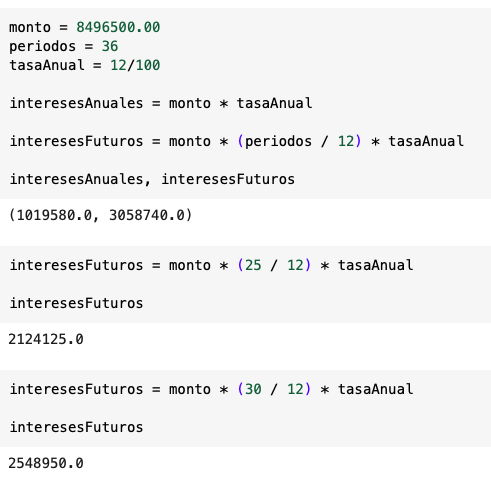
\includegraphics[width=\textwidth]{figures/s109-1.png}
    \end{minipage}
    \captionsetup{width=\textwidth}
    \caption{Código para calcular los intereses futuros}
    \label{fig:s109-1}
\end{figure}

\break
\noindent
En la Figura \ref{fig:s109-2} se muestra el código que calcula todos los intereses futuros, mes con mes, para determinar que los intereses superarán los \textbf{\$ 40,000.00} a partir del quinto mes. También se calcula la cuota fija que considera los intereses futuros y el descuento inicial al monto del \textbf{10\%}.
\begin{figure}[!ht]
    \centering
    \begin{minipage}{\textwidth}
        \centering
        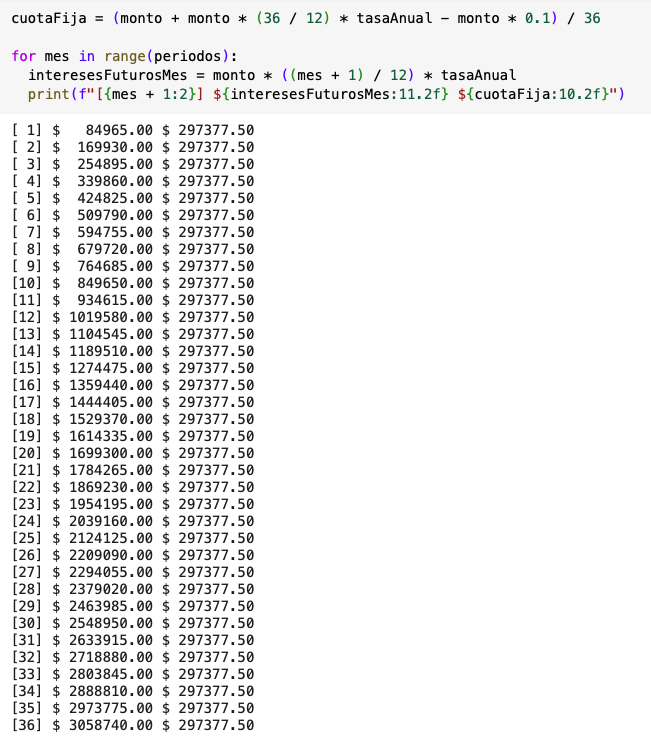
\includegraphics[width=\textwidth]{figures/s109-2.png}
    \end{minipage}
    \captionsetup{width=0.9\textwidth}
    \caption{Código para generar la tabla de intereses futuros mes por mes}
    \label{fig:s109-2}
\end{figure}

\clearpage

\subsection*{Problema 10 | Punto de Liquidación}

Un banco financió un proyecto durante 48 meses por \textbf{\$ 6,232,800.00}, con una tasa anual fija y simple del \textbf{12\%} y desea calcular el valor de liquidación que considere pagar los intereses futuros y la deuda total, la liquidación se llevará a cabo en el mes 28.
\\[12pt]
(a) Calcula los intereses totales.
\\[6pt]
(b) Calcula los intereses faltantes a partir del mes 28.
\\[6pt]
(c) Calcula la deuda de liquidación para el mes 28.

\clearpage

\subsubsection*{Solución al Problema 10}

En este problema nos pide calcular el punto de liquidación, que consiste en calcular los intereses futuros y la suma de cuotas pendientes a partir de cierto mes. En este caso queremos sumar los intereses futuros a partir del mes 29 hasta el mes 48 y las cuotas pendientes para hacer una liquidación. 
\\[12pt]
En la Figura \ref{fig:s110-1} se muestra el código que define el monto, periodos, tasa, mes de corte y resta de los meses faltantes, luego reporta el monto, el abono mensual, lo que se lleva pagado hasta el mes 28 y lo que se debe del monto hasta el mes 48 sin considerar los intereses. Observa que se calculan los montos pagados y la diferencia al monto total.
\begin{figure}[!ht]
    \centering
    \begin{minipage}{\textwidth}
        \centering
        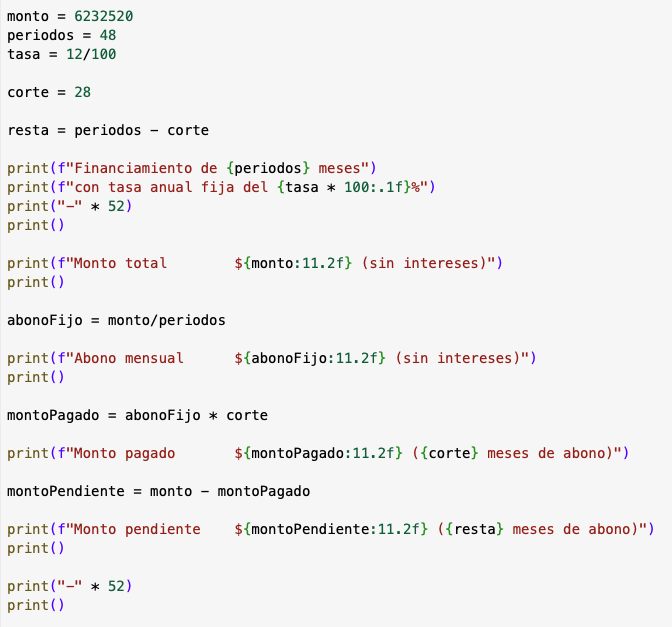
\includegraphics[width=\textwidth]{figures/s110-1.png}
    \end{minipage}
    \captionsetup{width=\textwidth}
    \caption{Código para reportar los montos futuros}
    \label{fig:s110-1}
\end{figure}

\break
\noindent
En la Figura \ref{fig:s110-2} se muestra el código que reporta ahora los intereses totales, los intereses mensuales, el interés pagado hasta el mes de corte y la diferencia entre el total y al corte que será el interés pendiente. Finalmente se calcula el monto de liquidación como lo pendiente entre el monto más los interés pendientes.
\begin{figure}[!ht]
    \centering
    \begin{minipage}{\textwidth}
        \centering
        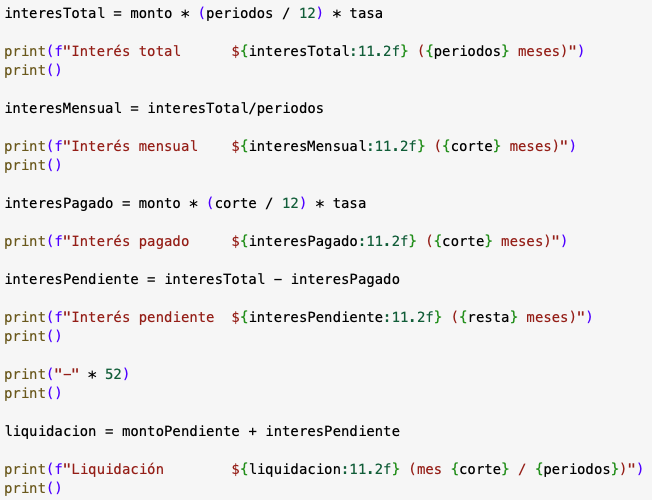
\includegraphics[width=\textwidth]{figures/s110-2.png}
    \end{minipage}
    \captionsetup{width=0.9\textwidth}
    \caption{Código para reportar los intereses futuros}
    \label{fig:s110-2}
\end{figure}

\break
\noindent
En la Figura \ref{fig:s110-3} se muestra el reporte generado que explica los montos e intereses hasta llegar al monto de liquidación.
\begin{figure}[!ht]
    \centering
    \begin{minipage}{\textwidth}
        \centering
        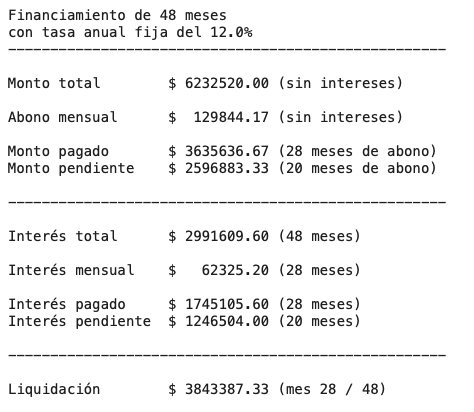
\includegraphics[width=\textwidth]{figures/s110-3.png}
    \end{minipage}
    \captionsetup{width=0.9\textwidth}
    \caption{Reporte de los montos e intereses y el punto de liquidación}
    \label{fig:s110-3}
\end{figure}

\clearpage

\section*{Módulo II | Estadística y Probabilidad con Python}

\subsection*{Problema 1 | Probabilidad de un Evento Simple} 

Una financiera posee una tabla con el género de sus clientes, si tiene trabajo, si está casado y si tiene alguna deuda.
\\[12pt]
En la Figura \ref{fig:p201} se muestra la tabla con el género, trabajo, casado y deuda de los clientes.
\begin{figure}[!ht]
    \centering
    \begin{minipage}{\textwidth}
        \centering
        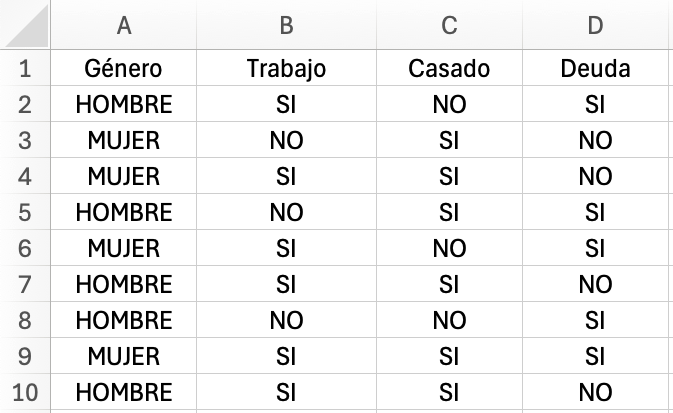
\includegraphics[width=\textwidth]{figures/p201.png}
    \end{minipage}
    \captionsetup{width=0.9\textwidth}
    \caption{Tabla de deuda por género, trabajo y casado}
    \label{fig:p201}
\end{figure}
\\
(a) Calcula la probabilidad de ser hombre
\\[6pt]
(b) Calcula la probabilidad de ser mujer
\\[6pt]
(c) Calcula la probabilidad de tener trabajo
\\[6pt]
(d) Calcula la probabilidad de no tener trabajo
\\[6pt]
(e) Calcula la probabilidad de estar casado
\\[6pt]
(f) Calcula la probabilidad de no estar casado
\\[6pt]
(g) Calcula la probabilidad de tener deuda
\\[6pt]
(h) Calcula la probabilidad de no tener deuda

\clearpage

\noindent
En la Figura \ref{fig:s201-1} se muestra el código que calcula las probabilidades, para los demás casos es similar.
\begin{figure}[!ht]
    \centering
    \begin{minipage}{\textwidth}
        \centering
        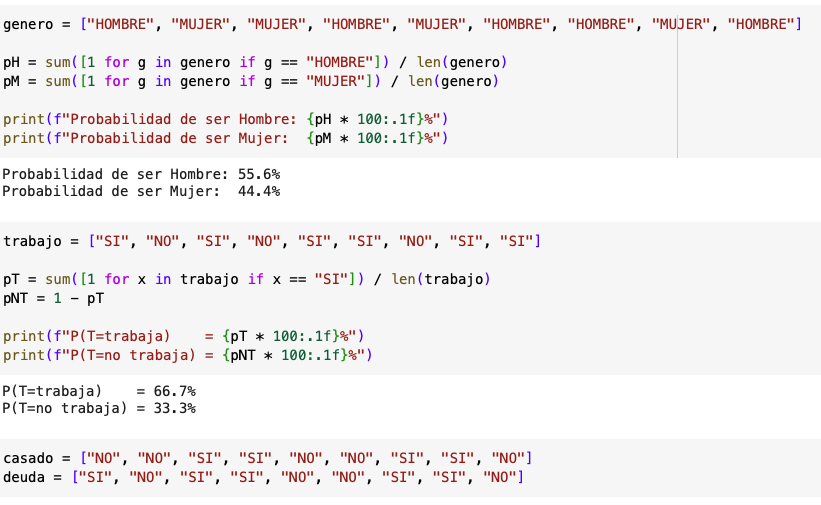
\includegraphics[width=\textwidth]{figures/s201-1.png}
    \end{minipage}
    \captionsetup{width=0.9\textwidth}
    \caption{Código para calcular la probabilidad simple por conteos}
    \label{fig:s201-1}
\end{figure}
\\
Observa que se filtran los elementos de la lista y se determina si el elemento de la lista cumple la condición, luego se coloca 1 en la nueva lista y se suman todos valores (la suma de los 1's dará el total), luego se divide por el número de elementos en la lista para determinar la probabilidad simple.

\clearpage

\subsection*{Problema 2 | Tabla conjunta de Dos Eventos}

Un restaurante está inspeccionando la bebidas asociadas al pago con tarjeta de sus clientes, porque sospecha que los clientes que pagan con tarjeta de crédito consumen más cerveza que aquellos que pagan con tarjeta de débito.
\\[12pt]
En la Figura \ref{fig:p202} se muestra la tabla con los datos de los clientes si utilizaron tarjeta de crédito o débito y el tipo de bebida que consumieron.
\begin{figure}[!ht]
    \centering
    \begin{minipage}{\textwidth}
        \centering
        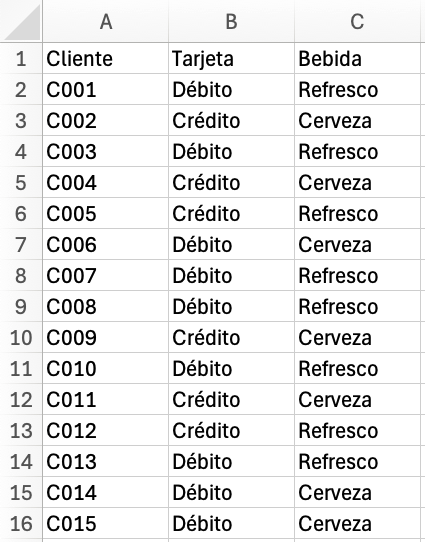
\includegraphics[width=0.9\textwidth]{figures/p202.png}
    \end{minipage}
    \captionsetup{width=0.9\textwidth}
    \caption{Tabla de tipo bebida consumida asociada al tipo de tarjeta}
    \label{fig:p202}
\end{figure}
\\

\break
\noindent
(a) Genera la tabla conjunta donde las filas sean el tipo de tarjeta (Débito, Crédito) y las columnas el tipo de bebida (Refresco, Cerveza). En cada celda pon el número total de registros que cumplen la fila y la columna, por ejemplo, para la fila Débito y la columna Refresco, hay 6 registros.
\\[6pt]
(b) Agrega una columna adicional con los totales marginales para la fila, sumando todas las columnas.
\\[6pt]
(c) Agrega una fila adicional para los totales marginales para la columna, sumando todas las filas.
\\[6pt]
(d) Indica el total de registros en la intersección de la columna marginal y la fila marginal.

\clearpage

\noindent
En la Figura \ref{fig:s202-1} se muestra el código que define los ejes de datos para las tarjetas y bebidas usando listas de python. Luego se crea una matriz de $2 \times 2$ usando listas para almacenar los conteos, después se calcula la suma de las parejas entre tarjetas y bebidas según la condición sobre la tarjeta $t$ y la bebida $b$, aquí se usa la lista generada que coloca un $1$ para cada tarjeta y bebida $(t, b)$ en la secuencia de embolsado $zip(X, Y)$ que recorre al mismo tiempo los elementos de $X$ y de $Y$, luego a esta lista de $1's$ se les callcula la suma y dicha suma será el total de elementos que cumplan ser una tarjeta y una bebida específica. En el índice $(0, 0)$ de la matriz se coloca cuántas tarjetas de Débito y bebida de refresco hubieron, similar para los demás. Finalmente se imprime la matriz de forma manual, mostrando las dos filas con sus dos columnas que representan las sumas y dejando los espacios necesarios para verse bien.
\begin{figure}[!ht]
    \centering
    \begin{minipage}{\textwidth}
        \centering
        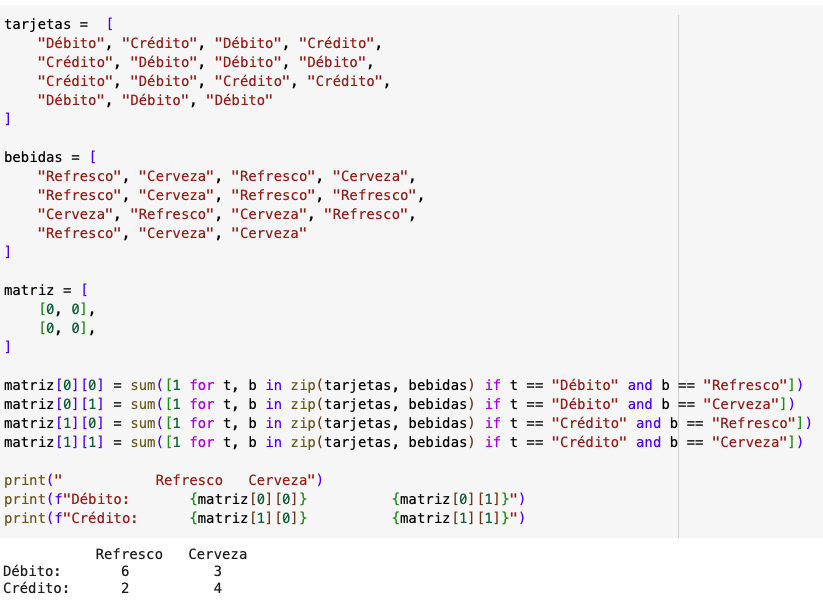
\includegraphics[width=\textwidth]{figures/s202-1.png}
    \end{minipage}
    \captionsetup{width=0.9\textwidth}
    \caption{Código para calcular la tabla conjunta entre dos eventos}
    \label{fig:s202-1}
\end{figure}
\\

\break
\noindent
En la Figura \ref{fig:s202-2} se muestra el código para calcular los marginales, el código comienza por agregar una columna más a la primera fila, conteniendo la suma de las columnas anteriores (la columna $0$ y $1$), luego se repite para agregar una columna más en la segunda fila, con la suma de los anteriores sobre la misma fila. Después se agrega una fila más a la matriz, con dos columnas, que contienen la suma de las filas anteiores (la fila $0$ y $1$). Luego se agrega una tercera columna a esta tercera fila marginal con la suma de las columnas anteriores, aunque sería equivalente usar la suma de las filas anteriores de la última columna. Finalmente se genera el reporte agregando algunos símbolos que mejoran el aspecto y considerando dos dígitos para la los valores de la última columna.
\begin{figure}[!ht]
    \centering
    \begin{minipage}{\textwidth}
        \centering
        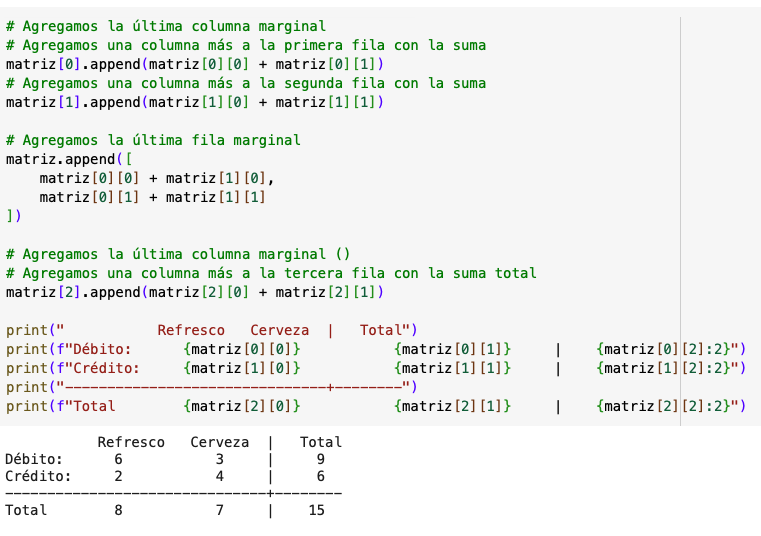
\includegraphics[width=\textwidth]{figures/s202-2.png}
    \end{minipage}
    \captionsetup{width=0.9\textwidth}
    \caption{Código para calcular los marginales en la tabla conjunta}
    \label{fig:s202-2}
\end{figure}
\\

\clearpage

\subsection*{Problema 3 | Probabilidad Conjunta de Dos Eventos}

Una empresa ha recuperado la tabla conjunta del personal que fue promovido a un mejor puesto y los que no a lo largo de 3 años. La tabla divide los hombres y mujeres contra si fueron o no promovidos, también cuenta con sus totales marginales. La empresa necesita encontrar la probabilidad conjunta de que los hombres hayan sido promividos o no.
\\[12pt]
En la Figura \ref{fig:p203} se muestra la tabla conjunta de promoción del personal por género.
\begin{figure}[!ht]
    \centering
    \begin{minipage}{\textwidth}
        \centering
        \includegraphics[width=\textwidth]{figures/p203.png}
    \end{minipage}
    \captionsetup{width=0.9\textwidth}
    \caption{Tabla conjunta de promoción del personal por género}
    \label{fig:p203}
\end{figure}
\\
(a) Divide cada valor de la tabla conjunta por el total marginal de $464$.
\\[6pt]
(b) Indica cual es la probabilidad total de que un hombre haya sido promovido.
\\[6pt]
(c) Indica cual es la probabilidad total de que un hombre no haya sido promovido.
\\[6pt]
(d) Indica cual es la probabilidad total de que una mujer haya sido promovida.
\\[6pt]
(e) Indica cual es la probabilidad total de que una mujer no haya sido promovida.
\\[6pt]
(f) Indica cual es la probabilidad total de que alguien sea hombre.
\\[6pt]
(g) Indica cual es la probabilidad total de que alguien sea mujer.
\\[6pt]
(h) Indica cual es la probabilidad total de que alguien sea promovido.
\\[6pt]
(i) Indica cual es la probabilidad total de que alguien no sea promovido.

\clearpage

\subsection*{Problema 4 | Probabilidad Condicional de Dos Eventos}

Una fábrica de cosméticos está diseñando un nuevo programa para que sus empleados trabajen dos horas menos de lo convencional. Para determinar si su modelo funciona, ha contratado empleados temporales, a los cuales se les pregunta si quieren ganar \textbf{\$ 2,800} por 6 horas diarias durante los 6 días de jornada de la semana, o ganar \textbf{\$ 4,080} por 8 horas. Al cabo de la semana, el empleado temporal tiene la oportunidad de tener un contrato de 3 meses o renunciar.
\\[12pt]
Después de construir la tabla conjunta con el número de empleados que trabajaron 6 horas u 8 horas y que renunciaron o no renunciaron, la empresa decide generar la tabla de probabilidad conjunta para no exponer los números netos sobre los empleados que contrató. Ahora requiere calcular la probabilidad de haber trabajado 6 horas dado que renunció y haber trabajado 8 horas dado que renunció, para poder entender cuál era turno que eligió una persona que decidió renunciar al final.
\\[12pt]
Además la empresa necesita saber cuál es la probabilidad de renunciar, dado que se trabaja 6 horas y la probabilidad de renunciar dado que se trabaja 8 horas, para entender quién tiene mayor probabilidad de renunciar y decidir si vale la pena mantener un turno de 8 horas en el futuro.
\\[12pt]
En la Figura \ref{fig:p204} se muestra la tabla de probabilidad de los empleados que deciden renunciar o no en turnos de 6 y 8 horas.
\begin{figure}[!ht]
    \centering
    \begin{minipage}{\textwidth}
        \centering
        \includegraphics[width=\textwidth]{figures/p204.png}
    \end{minipage}
    \captionsetup{width=0.9\textwidth}
    \caption{Tabla de probabilidad de renuncia por turno}
    \label{fig:p204}
\end{figure}
\\

\break
\noindent
(a) Indica cual es la probabilidad que alguien renuncie $P(Renuncia)$
\\[6pt]
(b) Indica la probabilidad de que alguien trabaje 6 horas $P(6h)$
\\[6pt]
(c) Indica la probabilidad de que alguien trabaje 8 horas $P(8h)$
\\[6pt]
(d) Indica la probabilidad de que alguien trabaje trabaje 6 horas y renuncie $P(6h \cap Renuncia)$
\\[6pt]
(e) Indica la probabilidad de que alguien trabaje trabaje 8 horas y renuncie $P(8h \cap Renuncia)$
\\[6pt]
(f) Calcula la probabilidad de trabajar 6 horas dado que se renuncia 
\\[6pt]
$P(6h|Renuncia) = \frac{P(6h \cap Renuncia)}{P(Renuncia)}$.
\\[6pt]
(g) Calcula la probabilidad de trabajar 8 horas dado que se renuncia
\\[6pt]
$P(8h|Renuncia) = \frac{P(8h \cap Renuncia)}{P(Renuncia)}$.
\\[6pt]
(h) Calcula la probabilidad de renunciar dado que se trabajó 6 horas 
\\[6pt]
$P(Renuncia|6h) = \frac{P(6h \cap Renuncia)}{P(6h)}$.
\\[6pt]
(i) Calcula la probabilidad de renunciar dado que se trabajó 6 horas 
\\[6pt]
$P(Renuncia|8h) = \frac{P(8h \cap Renuncia)}{P(8h)}$.

\clearpage

\subsection*{Problema 5 | Probabilidad Conjunta de Tres Eventos}

Para cuando tenemos tres eventos simultáneos, por ejemplo, A - poseer un género (hombre o mujer), B - conseguir un aumento (conseguirlo o no conseguirlo) y C - tipo de trabajo (administrativo, operativo, de diseño, gerencial). Nos lleva a la necesidad de separar los datos más allá de una tabla, para eso, necesitaremos ahora plantear los datos como una sucesión de filas y la frecuencia con la que ocurren las combinaciones de eventos.
\\[12pt]
Por ejemplo, la siguiente tabla muestra todas las combinaciones posibles de los eventos A, B y C en la primera columna y su frecuencia (número de eventos) que ocurrieron, algunos tienen cero ya que no hay registros que cumplan esas tres condiciones al mismo tiempo, como ser hombre, no conseguir un aumento y tener un trabajo gerencial.
\[
\begin{array}{|l|c|}
\hline
\textbf{Combinación de Eventos (A, B, C)} & \textbf{Frecuencia} \\
\hline
\text{Hombre, Consigue aumento, Administrativo} & 12 \\
\text{Hombre, Consigue aumento, Operativo} & 8 \\
\text{Hombre, Consigue aumento, Diseño} & 15 \\
\text{Hombre, Consigue aumento, Gerencial} & 6 \\
\text{Hombre, No consigue aumento, Administrativo} & 7 \\
\text{Hombre, No consigue aumento, Operativo} & 10 \\
\text{Hombre, No consigue aumento, Diseño} & 4 \\
\text{Hombre, No consigue aumento, Gerencial} & 0 \\
\text{Mujer, Consigue aumento, Administrativo} & 18 \\
\text{Mujer, Consigue aumento, Operativo} & 20 \\
\text{Mujer, Consigue aumento, Diseño} & 25 \\
\text{Mujer, Consigue aumento, Gerencial} & 10 \\
\text{Mujer, No consigue aumento, Administrativo} & 5 \\
\text{Mujer, No consigue aumento, Operativo} & 3 \\
\text{Mujer, No consigue aumento, Diseño} & 2 \\
\text{Mujer, No consigue aumento, Gerencial} & 0 \\
\hline
\end{array}
\]
Lugo para poder determinar la probabilidad conjunta de que ocurra un evento combinado, tendríamos que dividir cada frecuencia entre la suma.
\\[12pt]
(a) Calcula la probabilidad que ocurran los eventos dividiendo cada frecuencia entre la suma de todas las frecuencias.
\\[6pt]
(b) Indica la probabilidad de ser mujer, conseguir un aumento y ser administrativa.
\\[6pt]
(c) Indica la probabilidad de ser mujer, conseguir un aumento y ser de diseño.
\\[6pt]
(d) Indica la probabilidad de ser hombre, no conseguir un aumento y ser de administrativo.
\\[6pt]
(e) ¿Quién tiene mayor probabilidad de conseguir un aumento, hombres o mujeres?, ¿Cómo calculaste esta probabilidad?

\clearpage

\subsection*{Problema 6 | Probabilidad Condicional de Tres Eventos}

Para calcular la probabilidad condicional de tres eventos, necesitamos la tabla de probabilidad conjunta, y las tablas marginales de la probabilidad simple o combinada de que ocurran los eventos anteriores.
\\[12pt]
Por ejemplo, si se tienen tres eventos A, B y C y se desea calcular la probabilidad condicional $P(A=a_1|B=b_1,C=c_1)$ que se lee como la probabilidad que el evento A tenga el valor de $a_1$, dado que el evento B tiene el valor de $b_1$ y el evento C tenga el valor de $c_1$, entonces necesitaremos desarrollar la probabilidad con la regla de bayes como:
\begin{equation*}
    \begin{aligned}
        P(A=a_1|B=b_1,C=c_1) = \frac{P(A=a_1,B=b_1,C=c_1)}{P(B=b_1,C=c_1)}
    \end{aligned}
\end{equation*}
Pero, si desearmos calcular la probabilidad condicional $P(A=a_2,B=b_2|C=c_2)$ que se lee como la probabilidad que el evento A tenga el valor de $a_2$ y el evento B tiene el valor de $b_2$ (se desea saber la probabilidad que $A=a_2$ y $B=b_2$ pasen), dado que el evento C tenga el valor de $c_2$ (ya ocurrió que esto pasa), entonces necesitaremos desarrollar la probabilidad con la regla de bayes como:
\begin{equation*}
    \begin{aligned}
        P(A=a_1,B=b_1|C=c_1) = \frac{P(A=a_1,B=b_1,C=c_1)}{P(C=c_1)}
    \end{aligned}
\end{equation*}
Entonces, en resumen, estamos usando las probabilidades marginales $P(A=a)$, $P(B=b)$, $P(C=c)$, $P(A=a,B=b)$, $P(A=a,C=c)$, $P(B=b,C=c)$ y $P(A=a,B=b,C=c)$, lo que implica tener la probabilidad que ocurra cada posible valor en cada evento y las combinaciones. Es decir, tendremos una tabla como la del problema anterior donde tenemos cada valor de los eventos A, B y C y su probabilidad de que ocurra esa combinación, más a parte tendremos las tablas de probabilidad conjunta para los eventos $(A, B)$, $(A, C)$, $(B,C)$ y la tabla simple para cada posible valor del evento de $A$, del evento $B$ y del evento $C$.
\\[12pt]
Por lo que, tenemos las tablas de probabilidad conjunta y simple $(A,B,C)$, $(A,B)$, $(A,C)$, $(B,C)$, $(A)$, $(B)$, $(C)$.
\\[12pt]
Por ejemplo, supongamos los tres eventos que ocurren en la cafetería de una empresa: A - tipo de empleado (permanente, temporal), B - tipo de puesto (programación, diseño) y C - tipo de alimento preferido (saludable, no saludable). Entonces podemos formar todas las tablas de probabilidad conjunta, donde la primera columna indicará la combinación de valores sobre los eventos y la segunda columna la probabilidad que ocurra dicha combinación, tanto para los tres eventos simultáneos, como para sus combinaciones, entonces todas las tablas para este ejemplo son:
\\[12pt]
Probabilidad que ocurran los tres eventos (A, B, C):
\[
\begin{array}{|l|c|}
\hline
\textbf{Combinación de Eventos (A, B, C)} & \textbf{P(A,B,C)} \\
\hline
\text{Permanente, Programación, Saludable} & 0.12 \\
\text{Permanente, Programación, No saludable} & 0.08 \\
\text{Permanente, Diseño, Saludable} & 0.10 \\
\text{Permanente, Diseño, No saludable} & 0.05 \\
\text{Temporal, Programación, Saludable} & 0.15 \\
\text{Temporal, Programación, No saludable} & 0.10 \\
\text{Temporal, Diseño, Saludable} & 0.20 \\
\text{Temporal, Diseño, No saludable} & 0.10 \\
\hline
\end{array}
\]
Probabilidad que ocurran los dos eventos (A, B):
\[
\begin{array}{|l|c|}
\hline
\textbf{Combinación de Eventos (A, B)} & \textbf{P(A,B)} \\
\hline
\text{Permanente, Programación} & 0.20 \\
\text{Permanente, Diseño} & 0.15 \\
\text{Temporal, Programación} & 0.25 \\
\text{Temporal, Diseño} & 0.30 \\
\hline
\end{array}
\]
Probabilidad que ocurran los dos eventos (A, C):
\[
\begin{array}{|l|c|}
\hline
\textbf{Combinación de Eventos (A, C)} & \textbf{P(A,C)} \\
\hline
\text{Permanente, Saludable} & 0.22 \\
\text{Permanente, No saludable} & 0.13 \\
\text{Temporal, Saludable} & 0.35 \\
\text{Temporal, No saludable} & 0.20 \\
\hline
\end{array}
\]
Probabilidad que ocurran los dos eventos (B, C):
\[
\begin{array}{|l|c|}
\hline
\textbf{Combinación de Eventos (B, C)} & \textbf{P(B,C)} \\
\hline
\text{Programación, Saludable} & 0.27 \\
\text{Programación, No saludable} & 0.18 \\
\text{Diseño, Saludable} & 0.30 \\
\text{Diseño, No saludable} & 0.25 \\
\hline
\end{array}
\]
Probabilidad que ocurran los valores para el evento A:
\[
\begin{array}{|l|c|}
\hline
\textbf{A} & \textbf{P(A)} \\
\hline
\text{Permanente} & 0.35 \\
\text{Temporal} & 0.65 \\
\hline
\end{array}
\]
Probabilidad que ocurran los valores para el evento B:
\[
\begin{array}{|l|c|}
\hline
\textbf{B} & \textbf{P(B)} \\
\hline
\text{Programación} & 0.45 \\
\text{Diseño} & 0.55 \\
\hline
\end{array}
\]
Probabilidad que ocurran los valores para el evento C:
\[
\begin{array}{|l|c|}
\hline
\textbf{C} & \textbf{P(C)} \\
\hline
\text{Saludable} & 0.57 \\
\text{No saludable} & 0.43 \\
\hline
\end{array}
\]
Observa que las tablas marginales se derivan de sumar los eventos complementarios, por ejemplo, para calcular la tabla marginal de los eventos $(A, C)$, se sumaron las probabilidades de la tabla $(A,B,C)$ para todos los valores de $B$, en este caso, se dice que el evento $B$ fue reducido. Otro ejemplo, es que para calcular la tabla marginal del evento C, se tuvieron que reducir los evento $A$ y $B$ de la tabla $(A,B,C)$, es decir, sumar todas las probabilidades de A y B.
\\[12pt]
Ahora con estas tablas podemos resolver la probabilidad condicional que nos interese, por ejemplo, la probabilidad que alguien sea un programador, dado que es temporal y come comida saludable:
\begin{equation*}
    P(B=\text{programación}|A=\text{temporal},C=\text{saludable}) \\
\end{equation*}
\begin{equation*}
    \hspace*{2cm}
    \begin{aligned}
        &= \frac{P(A=\text{temporal},B=\text{programación},C=\text{saludable})}{P(A=\text{temporal},C=\text{saludable})} \\
        &= \frac{0.15}{0.35} \\
        &= 0.4286 \, (42.86\%)
    \end{aligned}
\end{equation*}
De esta forma solo basta con consultar las tablas e indicar la probabilidad que se tiene por ejemplo, $P(A=\text{temporal},C=\text{saludable}) = 0.35$ que se obtuvo de la tabla $(A, C)$ en los valores combinados.
\\[12pt]
Calcula las siguiente probabilidades:
\\[12pt]
(a) La probabilidad de comer saludable siendo programador temporal.
\\[6pt]
(b) La probabilidad de comer no saludable siendo diseñador permanente.
\\[6pt]
(c) La probabilidad de ser temporal siendo diseñador y no comer saludable.
\\[6pt]
(d) La probabilidad de permanente siendo programador que come saludable.

\clearpage

\subsection*{Problema 7 | Estadísticos Principales de Un Eje}

Los \textbf{estadísticos principales} de un eje de datos permiten analizar y describir el comportamiento de los valores registrados en dicho eje. Un eje de datos puede considerarse como una variable aleatoria cuyos valores comparten una lógica subyacente, lo que los hace pertenecer a la misma categoría de análisis. Por ejemplo, un eje que contiene las edades de una muestra, o uno que describe el grado académico alcanzado por una población.
\\[12pt]
Generalmente, el eje de datos representa valores observados de una muestra tomada de la población de interés. Estos datos contienen información que, a través del análisis estadístico, permite inferir propiedades del conjunto. Es importante diferenciar entre los términos \textbf{estadística y estadístico}:
\begin{itemize}
    \item \textbf{Estadística}: hace referencia al campo de estudio o al conjunto de métodos utilizados para analizar los datos.
    \item \textbf{Estadístico}: es un valor calculado a partir de los datos de una muestra, como la media, la mediana o los percentiles, que describe una característica específica de la muestra.
\end{itemize}
En este contexto, nos referimos a \textbf{estadísticos} como los resultados de aplicar procedimientos matemáticos a los datos (por ejemplo, el cálculo de la mediana o un percentil). Estos estadísticos se utilizan para describir y resumir los datos, permitiendo generar una \textbf{estadística descriptiva} que facilite la interpretación de las propiedades del eje de datos respecto a la población analizada.
\\[12pt]
Dentro de los estadísticos, algunos se consideran principales porque son ampliamente utilizados para describir datos de manera práctica y efectiva. Estos estadísticos permiten realizar análisis descriptivos que, a partir de una muestra, nos acercan a una comprensión más general sobre la población en estudio.
\\[12pt]
Los estadísticos principales son:
\begin{itemize}
    \item \textbf{Conteo} - Representa el total de elementos en la muestra, generalmente se llama $N$ o $n$ y se asocia algunas veces a los grados de libertad, por ejemplo, algunas distibuciones usan $n-1$ grados de libertad para hacer cálculos como la prueba $F$.
    \item \textbf{Suma} - Representa la suma de todos los valores del eje y explica la dimesión o volumen del eje, por ejemplo, si cada dato en el eje es un precio de algún producto, la suma representará la cantidad total de dinero acumulado en todos los productos.
    \item \textbf{Mínimo} - Representa el valor mínimo dentro de todos los datos, este valor explica el límite inferior alcanzado por los datos, por ejemplo, si el eje de datos son estaturas, explicará cuál es la estatura más pequeña registrada.
    \item \textbf{Máximo} - Representa el valor máximo dentro de todos los datos, este valor explica el límite superior alcanzado por los datos, por ejemplo, si el eje de datos son pesos, explicará cuál es el peso más grande registrado.
    \item \textbf{Promedio / Media} - Representa el valor más cercano a todos los valores dentro del eje, esta valor explica el valor ideal que deberían tener todos los datos si se reducieran a un único valor, por ejemplo, si el eje de datos son salarios, el promedio representaría el salario que deberían tener todos si ganaran lo mismo y cuya suma se mantendría.
    \item \textbf{Cuartil 1 / $Q_1 \sim 25\%$} - Representa el valor que separa el primer $25\%$ de los datos ordenados respecto al resto ($75\%$). Este valor indica el límite superior de los datos más bajos en la distribución, lo que puede ser útil para identificar valores considerados significativamente pequeños. Por ejemplo, si los datos corresponden a fallas en motores de automóviles, el primer cuartil reflejará el número de fallas acumuladas en el $25\%$ de los vehículos con menor número de fallas.
    \item \textbf{Cuartil 2 / $Q_2 \sim 50\%$ / Mediana} - Representa el valor que divide los datos en dos mitades iguales, es decir, el $50\%$ de los valores inferiores y el $50\%$ de los valores superiores. Este estadístico mide el valor central de la distribución y puede usarse para identificar sesgos en los datos. Por ejemplo, si los datos son tiempos de fabricación de una pieza, el segundo cuartil o mediana refleja el tiempo intermedio, indicando si la distribución de tiempos está más próxima a $Q_1$ o $Q_3$.
    \item \textbf{Cuartil 3 / $Q_3 \sim 75\%$} - Representa el valor que separa el $75\%$ de los datos ordenados respecto al $25\%$ restante. Este valor marca el límite inferior de los datos más altos en la distribución y puede ser útil para identificar valores significativamente grandes. Por ejemplo, si los datos corresponden al índice de madurez de manzanas (verde o roja), el tercer cuartil representará el valor alcanzado por el $75\%$ de las manzanas con mayor madurez.
    \item \textbf{Percentil 5\% / $P_{5} \sim 5\%$ / Mínimo relativo} - Representa el valor que corta el $5\%$ inferior de los datos ordenados de menor a mayor. Este estadístico ayuda a evitar que valores extremos (outliers) distorsionen los análisis, proporcionando un límite inferior más confiable que el mínimo absoluto. Por ejemplo, si los datos son alturas de tornillos producidos, el percentil $5\%$ excluiría tornillos con alturas inusualmente bajas, posiblemente debidas a errores de medición.
    \item \textbf{Percentil 95\% / $P_{95} \sim 95\%$ / Máximo relativo} - Representa el valor que corta el $5\%$ superior de los datos ordenados de mayor a menor. Este estadístico establece un límite superior confiable, ignorando valores atípicos o errores de medición que podrían sesgar el máximo absoluto. Por ejemplo, si los datos son tiempos de permanencia de clientes en una sucursal, el percentil $95\%$ excluiría tiempos extremadamente largos registrados en situaciones atípicas.
\end{itemize}
El siguiente ejemplo muestra un eje de datos sobre los precios de la gasolina a lo largo del mes de enero con 31 valores representan el precio que fue registrado día a día, por ejemplo el día 1 el precio fue de \textbf{\$ 23.65} y el día 18 de \textbf{\$ 24.16}.
\begin{table}[ht]
    \centering
    \caption{Precios de la Gasolina a lo Largo del Mes}
    \begin{tabular}{|c|c|}
        \hline
        \textbf{Día} & \textbf{Precio (en \$)} \\
        \hline
        1 & 23.65 \\
        2 & 23.75 \\
        3 & 23.85 \\
        4 & 23.90 \\
        5 & 24.00 \\
        6 & 24.10 \\
        7 & 24.05 \\
        8 & 24.15 \\
        9 & 24.25 \\
        10 & 24.30 \\
        11 & 24.35 \\
        12 & 24.40 \\
        13 & 24.45 \\
        14 & 24.50 \\
        15 & 24.55 \\
        16 & 24.60 \\
        17 & 24.65 \\
        18 & 24.16 \\
        19 & 24.20 \\
        20 & 24.25 \\
        21 & 24.30 \\
        22 & 24.35 \\
        23 & 24.40 \\
        24 & 24.45 \\
        25 & 24.50 \\
        26 & 24.55 \\
        27 & 24.60 \\
        28 & 24.65 \\
        29 & 24.70 \\
        30 & 24.75 \\
        31 & 24.80 \\
        \hline
    \end{tabular}
\end{table}
\\
(a) Determina los estadísticos principales descritos.
\\[6pt]
(b) ¿Qué tan alejado está el mínimo absoluto del relativo?
\\[6pt]
(c) ¿Qué tan alejado está el máximo absoluto del relativo?

\clearpage

\subsection*{Problema 8 | Estadísticos Principales de Dos Ejes }

Cuando analizamos dos ejes, es muy común agregar cuatro estadísticos principales más para poder comparar el comportamiento entre los ejes, estos son:
\begin{itemize}
    \item \textbf{Varianza} - Representa qué tan alejados cuadráticamente están los valores de la media.
    \item \textbf{Desviación Estándar} - Representa qué tan alejados están los valores de la media en la misma magnitud, este se calcula como la raíz cuadrada de la varianza.
    \item \textbf{Covarianza} - Representa qué tan alejados están los valores de un eje respecto a su media del eje y los valores del otro eje respecto a la media de ese otro eje, es decir, mide el grado de dispersión entre dos ejes, este será positivo si al mismo tiempo los valores de un eje son mayores a su media, mientras que los valores del otro eje también son mayores a su media o al mismo tiempo ambos son menores a la media de su respectivo eje, ya que el producto será positivo. En el caso que uno sea mayor a su media y el otro menor o viceversa, el producto será negativo y la suma de todas las ponderaciones será negativo, finalmente será cero si las sumas se anulan por a veces ser positivas o negativas. La covarianza mide la relación entre dos ejes y esta relación es positiva o directa si la suma de las ponderaciones es muy positiva, la relación será negativa o inversa si las ponderaciones son muy negativas o la relación será cero o nula si se anulan.
    \item \textbf{Correlación} - Representa el grado de relación entre $[-1, 1]$ y se obtiene de normalizar la covarianza mediante la desviación de cada eje.
\end{itemize}
Podemos comparar dos ejes estadísticamente para entender qué tan similares o distintos son comparando sus medias y el grado de correlación entre ambos ejes. Si la correlación es cercana $1$ diremos que un eje explica al otro y viceversa de forma directa, es decir, cuando los valores de un eje crecen, los valores en el otro eje también lo hacen. Si la correlación es cercana a $-1$ diremos que un eje explica al otro y viceversa de forma inversa, es decir, cuando los valores de un eje crecen, los valores en el otro eje decrecen (al revés). Y si la correlación es cercana a $0$, diremos que un eje no explica al otro y viceversa, es decir hay una relación nula entre ambos ejes.
\\[12pt]
Por ejemplo, podemos comparar dos ejes de datos estadísticamente, para determinar si hay una correlación entre sus datos que nos lleven a concluir si un eje es capaz de explicar al otro. Tomemos las estaturas y pesos que se medieron de 15 personas y determinemos el grado de relación entre la estatura y el peso. La correlación entre el eje de datos de las estaturas y el eje de datos de los pesos determinará si la relación es directa, inversa o nula, de ser directa, a mayor estatura se encontrará un mayor peso (o a menor estatura, menor peso), al ser inversa a menor estatura mayor será el peso (o a mayor estatura, menor peso) o al ser nula, no se encontrará una relación entre las estaturas y los pesos.
\begin{table}[ht]
    \centering
    \caption{Precios de la Gasolina a lo Largo del Mes}
    \begin{tabular}{|c|c|}
        \hline
        \textbf{Estatura (m)} & \textbf{Peso (kg)} \\
        \hline
        1.67 & 65 \\
        1.58 & 56 \\
        1.72 & 78 \\
        1.68 & 63 \\
        1.53 & 61 \\
        1.65 & 71 \\
        1.84 & 95 \\
        1.49 & 56 \\
        1.57 & 52 \\
        1.91 & 87 \\
        1.83 & 84 \\
        1.67 & 70 \\
        1.70 & 64 \\
        1.58 & 48 \\
        1.82 & 95 \\
        \hline
    \end{tabular}
\end{table}
\\
(a) Calcula la media de las estaturas
\\[6pt]
(b) Calcula la media de los pesos
\\[6pt]
(c) Calcula la varianza de las estaturas
\\[6pt]
(d) Calcula la varianza de los pesos
\\[6pt]
(e) Calcula la desviación estándar de las estaturas
\\[6pt]
(f) Calcula la desviación estándar de los pesos
\\[6pt]
(g) Calcula la covarianza entre estaturas y pesos
\\[6pt]
(h) Calcula la correlación entre estaturas y pesos
\\[6pt]
(i) Indica que tipo de relación es la correlación

\clearpage

\subsection*{Problema 9 | Matriz de Correlación entre Tres Ejes}

Diseña una matriz de correlación que considere 3 ejes, la correlación está definida 2 a 2. Por lo que tendrás que considerar que las filas serán los 3 ejes y las columnas también los 3 ejes, luego en cada celda entre la fila y la columna anota la correlación entre el eje de la fila y el eje de la columna. Observa que sea cual sea el eje, la diagonal de la matriz será 1 dado que la correlación entre el eje y el mismo es 1 siempre.
\\[12pt]
Por ejemplo, para los ejes de datos A, B, C tendríamos:
\begin{table}[ht]
    \centering
    \caption{Precios de la Gasolina a lo Largo del Mes}
    \begin{tabular}{|l|c|c|c|}
        \hline
        - & \textbf{A} & \textbf{B} & \textbf{C} \\
        \hline
        \textbf{A} & 1 & · & · \\
        \textbf{B} & · & 1 & · \\
        \textbf{C} & · & · & 1 \\
        \hline
    \end{tabular}
\end{table}
\\
(a) Diseña 3 ejes de datos con al menos 10 valores realistas cada uno
\\[6pt]
(b) Genera la matriz de correlación entre los 3 ejes, calculando la correlación entre el eje de la fila y el eje de la columna
\\[6pt]
(c) Indica si el segundo o tercer eje de datos tiene mayor correlación hacia el primer eje de datos, ya sea positiva o negativa
\\[6pt]
(d) Ubica el valor de mayor correlación que no esté en la diagonal
\\[6pt]
(e) Describe la hipótesis sobre esta correlación según si su relación es directa, inversa o nula

\clearpage

\subsection*{Problema 10 | Prueba F entre Dos Hipótesis de Un Eje}

Diseña un experimento que considere dos ejes de datos de una misma característica de la población objetivo, pero para diferentes segmentos de la población. Por ejemplo, si la población son precios de productos, toma el primer eje de datos como los precios de los productos que se venden más en línea y el otro eje de datos como los precios de los productos que venden más en tienda física. Otro ejemplo, es la población de personas que fuman, considera un eje de datos bajo el segmento de los que son hombres y el otro eje de datos como las personas que son mujeres.
\\[12pt]
Los ejes no necesariamente deben tener el mismo número de elementos, por ejemplo, un eje podría tener 60 precios de productos, mientras que el otro eje de datos podría contener solo 40 precios de productos.
\\[12pt]
(a) Diseña una población de una sola característica que se pueda segmentar fácilmente en dos segmentos
\\[6pt]
(b) Crea dos ejes de datos para el primer segmento, con al menos 20 valores realistas
\\[6pt]
(c) Calcula la media del primer eje
\\[6pt]
(d) Calcula la media del segundo eje
\\[6pt]
(e) Calcula la desviación estándar del primer eje
\\[6pt]
(f) Calcula la desviación estándar del segundo eje
\\[6pt]
(g) Calcula la covarianza entre ambos ejes
\\[6pt]
(h) Calcula la correlación entre ambos ejes
\\[6pt]
(i) Indica si la correlación es cercana a 1, 0, -1 y el tipo de relación
\\[6pt]
(j) Aplica la prueba F entre ambos ejes con $n_1-1$ grados de libertad para el primer eje y $n_2-1$ grados de libertad para el segundo eje. Donde $n_1, n_2$ son el número de elementos en el primer y segundo eje respectivamente
(k) Indica si el valor F es mayor a $0.05$ o no lo es y qué significa esto

\clearpage

\section*{Módulo III | Ciencia de Datos}

\subsection*{Problema 1 | Estructuración de un Dataset en Excel}

Crea un archivo Excel que represente la siguiente información:

\begin{table}[h]
    \centering
    \begin{tabular}{|c|c|c|c|}
        \hline
        País & Año & Población (millones) & PIB per cápita (USD) \\
        \hline
        México & 2022 & 126 & 10000 \\
        Estados Unidos & 2022 & 331 & 63000 \\
        Canadá & 2022 & 38 & 48000 \\
        Brasil & 2022 & 213 & 7500 \\
        Japón & 2022 & 126 & 40000 \\
        \hline
    \end{tabular}
    \caption{Datos para estructurar}
\end{table}

Guarda el archivo con el nombre \texttt{indicadores.xlsx}.

\clearpage

\subsection*{Problema 2 | Dataset de indicadores en CSV}

Convierte el archivo \texttt{indicadores.xlsx} del Problema 1 en un archivo CSV llamado \texttt{indicadores.csv}. Usa el siguiente formato de columnas:

\begin{verbatim}
País,Año,Población,PIB_per_capita
México,2022,126,10000
Estados Unidos,2022,331,63000
Canadá,2022,38,48000
Brasil,2022,213,7500
Japón,2022,126,40000
\end{verbatim}

\clearpage

\subsection*{Problema 3 | Adquisición de un CSV en Python}

Escribe un script en Python que lea el archivo \texttt{indicadores.csv} del Problema 2 y lo muestre en la consola. Completa el siguiente código:

\begin{lstlisting}[style=python]
import pandas as pd

# Ruta del archivo
file_path = "..."

# Cargar el CSV
df = pd.read_csv(file_path)

# Mostrar el DataFrame
print(...)
\end{lstlisting}

\clearpage

\subsection*{Problema 4 | Indicadores en Series de Pandas}

Usando el DataFrame cargado en el Problema 3, crea una Serie con los valores del PIB per cápita. Completa el siguiente código:

\begin{lstlisting}[style=python]
# Crear la Serie
pib_per_capita = ...

# Mostrar la Serie
print(pib_per_capita)
\end{lstlisting}

\clearpage

\subsection*{Problema 5 | Indicadores en DataFrames de Pandas}

Agrega una nueva columna llamada \texttt{PIB\_total} que calcule el PIB total como el producto de \texttt{Población} y \texttt{PIB per cápita}. Completa el código:

\begin{lstlisting}[style=python]
# Agregar la columna
df['PIB_total'] = ...

# Mostrar el DataFrame
print(df)
\end{lstlisting}

\clearpage

\subsection*{Problema 6 | Filtrar columnas en DataFrames}

Filtra únicamente las columnas \texttt{País} y \texttt{PIB\_total}. Completa el código:

\begin{lstlisting}[style=python]
# Filtrar columnas
filtered_df = df[...]

# Mostrar las columnas filtradas
print(filtered_df)
\end{lstlisting}

\clearpage

\subsection*{Problema 7 | Filtrar filas en DataFrames}

Filtra las filas donde el PIB total sea mayor a 1 billón de USD (\texttt{1e12}). Completa el código:

\begin{lstlisting}[style=python]
# Filtrar filas
high_pib = df[...]

# Mostrar las filas filtradas
print(high_pib)
\end{lstlisting}

\clearpage

\subsection*{Problema 8 | Agrupación de datos en DataFrames}

Agrupa los datos por año y calcula el promedio de PIB per cápita. Completa el código:

\begin{lstlisting}[style=python]
# Agrupar y calcular promedio
average_pib = df.groupby(...)[...].mean()

# Mostrar el resultado
print(average_pib)
\end{lstlisting}

\clearpage

\subsection*{Problema 9 | Combinación de datos en DataFrames}

Combina el DataFrame actual con otro que contenga información adicional, como índice de desarrollo humano (IDH). Completa el código:

\begin{lstlisting}[style=python]
# Crear otro DataFrame
idh_data = {
    "Pais": ["Mexico", "Estados Unidos", "Canada", "Brasil", "Japon"],
    "IDH": [0.758, 0.926, 0.929, 0.765, 0.919]
}
idh_df = pd.DataFrame(idh_data)

# Combinar DataFrames
combined_df = pd.merge(df, idh_df, on=...)

# Mostrar el resultado
print(combined_df)
\end{lstlisting}

\clearpage

\subsection*{Problema 10 | Visualización de datos}

Crea un gráfico de barras que muestre el PIB total por país usando la librería \texttt{matplotlib}. Completa el código:

\begin{lstlisting}[style=python]
import matplotlib.pyplot as plt

# Crear grafico de barras
plt.bar(..., ...)

# Configurar etiquetas
plt.xlabel("Pais")
plt.ylabel("PIB Total (USD)")
plt.title("PIB Total por Pais")

# Mostrar grafico
plt.show()
\end{lstlisting}

\section*{Módulo IV | Machine Learning}


% Problema 1
\subsection*{Problema 1 | Aprendizaje Supervisado}

Dado el siguiente conjunto de datos en formato CSV:

\begin{verbatim}
Edad,Salario,Compra
25,50000,No
35,60000,Sí
45,80000,Sí
30,70000,No
40,85000,Sí
\end{verbatim}

Carga estos datos en un DataFrame de pandas y utiliza la librería \texttt{sklearn} para entrenar un modelo de clasificación que prediga si una persona comprará un producto basado en su edad y salario.

\begin{lstlisting}[style=python]
from sklearn.model_selection import train_test_split
from sklearn.tree import DecisionTreeClassifier
import pandas as pd

# Cargar los datos
data = ...

# Separar variables independientes y dependientes
X = ...
y = ...

# Dividir los datos en conjuntos de entrenamiento y prueba
X_train, X_test, y_train, y_test = train_test_split(...)

# Entrenar el modelo
model = DecisionTreeClassifier()
model.fit(...)

# Evaluar el modelo
accuracy = model.score(...)
print(f"Accuracy: {accuracy}")
\end{lstlisting}

\clearpage

% Problema 2
\subsection*{Problema 2 | Regresión Simple}

Usa el siguiente conjunto de datos para predecir el precio de una casa basado en su tamaño en pies cuadrados:

\begin{verbatim}
Tamaño,Precio
1000,150000
1500,200000
2000,250000
2500,300000
3000,350000
\end{verbatim}

Crea un modelo de regresión lineal y muestra la ecuación de la recta ajustada.

\begin{lstlisting}[style=python]
from sklearn.linear_model import LinearRegression

# Datos
X = ...
y = ...

# Crear modelo
model = LinearRegression()
model.fit(...)

# Mostrar ecuacion de la recta
print(f"Coeficiente: {model.coef_}")
print(f"Intercepto: {model.intercept_}")
\end{lstlisting}

\clearpage

% Problema 3
\subsection*{Problema 3 | Regresión Múltiple}

Amplía los datos del Problema 2 agregando una columna de número de habitaciones:

\begin{verbatim}
Tamaño,Habitaciones,Precio
1000,2,150000
1500,3,200000
2000,4,250000
2500,4,300000
3000,5,350000
\end{verbatim}

Entrena un modelo de regresión múltiple para predecir el precio de una casa.

\clearpage

% Problema 4
\subsection*{Problema 4 | Clasificación Simple}

Utilizando el conjunto de datos del Problema 1, usa una regresión logística para predecir la compra de un producto.

\begin{lstlisting}[style=python]
from sklearn.linear_model import LogisticRegression

# Crear modelo
model = LogisticRegression()
model.fit(...)

# Prediccion
pred = model.predict(...)
print(f"Predicciones: {pred}")
\end{lstlisting}

\clearpage

% Problema 5
\subsection*{Problema 5 | Clasificación Múltiple}

Dado el siguiente conjunto de datos, crea un modelo de clasificación que prediga la categoría del cliente (A, B o C) basado en el ingreso y la edad:

\begin{verbatim}
Edad,Ingreso,Categoría
25,30000,A
35,50000,B
45,70000,C
30,40000,A
40,60000,B
\end{verbatim}

\clearpage

% Problema 6
\subsection*{Problema 6 | Aprendizaje No Supervisado}

Usa el siguiente conjunto de datos para aplicar el algoritmo de K-Means y agrupar los puntos en 2 clústeres:

\begin{verbatim}
X,Y
1,2
2,1
3,4
5,6
6,5
\end{verbatim}

\begin{lstlisting}[style=python]
from sklearn.cluster import KMeans

# Datos
X = ...

# Crear modelo
kmeans = KMeans(n_clusters=2)
kmeans.fit(...)

# Mostrar centroides
print(f"Centroides: {kmeans.cluster_centers_}")
\end{lstlisting}

\clearpage

% Problema 7
\subsection*{Problema 7 | Reducción de Dimensionalidad}

Aplica PCA (Análisis de Componentes Principales) a un dataset con 3 dimensiones y reduce el espacio a 2 dimensiones. Usa datos sintéticos generados con \texttt{numpy}.

\clearpage

% Problema 8
\subsection*{Problema 8 | Matriz de Adyacencia}

Crea una matriz de adyacencia que represente el siguiente grafo:

\[
A \leftrightarrow B, \; A \leftrightarrow C, \; B \leftrightarrow D, \; C \leftrightarrow D
\]

\begin{lstlisting}[style=python]
import numpy as np

# Matriz de adyacencia
adj_matrix = np.array([
    [0, 1, 1, 0],
    [1, 0, 0, 1],
    [1, 0, 0, 1],
    [0, 1, 1, 0]
])

print(adj_matrix)
\end{lstlisting}

\clearpage

% Problema 9
\subsection*{Problema 9 | Matriz de Similitud}

Dado un conjunto de puntos en un espacio 2D, calcula una matriz de similitud basada en la distancia euclidiana inversa.

\clearpage

% Problema 10
\subsection*{Problema 10 | Clusterización}

Aplica el algoritmo DBSCAN para encontrar clústeres en el siguiente conjunto de datos:

\begin{verbatim}
X,Y
1,2
2,2
3,3
8,8
8,9
25,30
\end{verbatim}

\begin{lstlisting}[style=python]
from sklearn.cluster import DBSCAN

# Datos
X = ...

# Aplicar DBSCAN
dbscan = DBSCAN(eps=2, min_samples=2)
dbscan.fit(...)

# Mostrar etiquetas de cluster
print(f"Etiquetas: {dbscan.labels_}")
\end{lstlisting}

\clearpage

\section*{Módulo IV | Deep Learning}

% Problema 1
\subsection*{Problema 1 | Modelo Generalizado}

Construye un modelo generalizado con Keras que tenga:

- Una capa de entrada con 10 neuronas.
- Una capa oculta con 16 neuronas y activación ReLU.
- Una capa de salida con una sola neurona y activación sigmoidal.

\begin{lstlisting}[style=python]
from keras.models import Sequential
from keras.layers import Dense

# Crear el modelo
model = Sequential([
    Dense(16, activation='relu', input_shape=(10,)),
    ...
])

# Compilar el modelo
model.compile(optimizer='adam', loss='binary_crossentropy', metrics=['accuracy'])
\end{lstlisting}

\clearpage

% Problema 2
\subsection*{Problema 2 | Perceptrón Simple}

Implementa un perceptrón simple para resolver el problema lógico AND:

\begin{verbatim}
Input: [0,0], [0,1], [1,0], [1,1]
Output: [0, 0, 0, 1]
\end{verbatim}

\begin{lstlisting}[style=python]
import numpy as np
from keras.models import Sequential
from keras.layers import Dense

# Datos
X = np.array([[0,0], [0,1], [1,0], [1,1]])
y = np.array([[0], [0], [0], [1]])

# Modelo
model = Sequential([
    Dense(1, activation='sigmoid', input_shape=(2,))
])

model.compile(optimizer='sgd', loss='binary_crossentropy', metrics=['accuracy'])

# Entrenar
model.fit(X, y, epochs=100, verbose=1)
\end{lstlisting}

\clearpage

% Problema 3
\subsection*{Problema 3 | Capa de Perceptrones Múltiples}

Crea un modelo con tres capas densas: la primera de 8 neuronas, la segunda de 4 neuronas, y la tercera de 2 neuronas, todas con activación ReLU.

\begin{lstlisting}[style=python]
model = Sequential([
    Dense(8, activation='relu', input_shape=(10,)),
    Dense(4, activation='relu'),
    Dense(2, activation='relu')
])
\end{lstlisting}

\clearpage

% Problema 4
\subsection*{Problema 4 | Modelo Secuencial Simple}

Entrena un modelo secuencial para predecir el precio de una casa basada en el tamaño:

\begin{verbatim}
Tamaño (m²): [50, 60, 70, 80, 90]
Precio (USD): [100, 120, 140, 160, 180]
\end{verbatim}

\begin{lstlisting}[style=python]
X = np.array([[50], [60], [70], [80], [90]])
y = np.array([[100], [120], [140], [160], [180]])

model = Sequential([
    Dense(1, activation='linear', input_shape=(1,))
])

model.compile(optimizer='sgd', loss='mean_squared_error')
model.fit(X, y, epochs=100, verbose=1)
\end{lstlisting}

\clearpage

% Problema 5
\subsection*{Problema 5 | Capas Densas Ocultas}

Modifica el modelo del problema 4 para agregar una capa oculta con 10 neuronas y activación ReLU.

\clearpage

% Problema 6
\subsection*{Problema 6 | Regresión Generalizada}

Entrena un modelo para realizar una regresión en el siguiente conjunto de datos:

\begin{verbatim}
X: [1, 2, 3, 4, 5]
y: [2.1, 4.2, 6.3, 8.4, 10.5]
\end{verbatim}

Ajusta la salida usando una función de pérdida \texttt{mean\_absolute\_error}.

\clearpage

% Problema 7
\subsection*{Problema 7 | Clasificación Generalizada}

Usa un modelo de clasificación para identificar si un punto en el plano pertenece al primer cuadrante. Los datos son:

\begin{verbatim}
X: [(1,1), (-1,1), (1,-1), (-1,-1)]
y: [1, 0, 0, 0]
\end{verbatim}

Entrena el modelo usando activación sigmoidal y optimizador Adam.

\clearpage

% Problema 8
\subsection*{Problema 8 | Exportación de una Red Neuronal}

Guarda el modelo creado en el Problema 7 en un archivo llamado \texttt{modelo.h5}.

\begin{lstlisting}[style=python]
model.save('modelo.h5')
\end{lstlisting}

\clearpage

% Problema 9
\subsection*{Problema 9 | Importación de una Red Neuronal}

Carga el modelo guardado en el Problema 8 y realiza predicciones en los datos:

\begin{lstlisting}[style=python]
from keras.models import load_model

# Cargar modelo
model = load_model('modelo.h5')

# Predicciones
pred = model.predict([[1,1]])
print(pred)
\end{lstlisting}

\clearpage

% Problema 10
\subsection*{Problema 10 | Predicción y Evaluación}

Evalúa el modelo del Problema 9 usando los siguientes datos de prueba:

\begin{verbatim}
X_test: [(1,1), (0,0), (-1,-1)]
y_test: [1, 0, 0]
\end{verbatim}

\begin{lstlisting}[style=python]
# Evaluar modelo
loss, accuracy = model.evaluate(X_test, y_test)
print(f"Loss: {loss}, Accuracy: {accuracy}")
\end{lstlisting}

\end{document}